% ------------------------------------------------------------
% LaTeX Template für die DHBW zum Schnellstart!
% Original: https://github.wdf.sap.corp/vtgermany/LaTeX-Template-DHBW
% ------------------------------------------------------------
% ---- Präambel mit Angaben zum Dokument
\documentclass[
	fontsize=12pt,           % Leitlinien sprechen von Schriftgröße 12.
	paper=A4,
	twoside=false,
	listof=totoc,            % Tabellen- und Abbildungsverzeichnis ins Inhaltsverzeichnis
	bibliography=totoc,      % Literaturverzeichnis ins Inhaltsverzeichnis aufnehmen
	titlepage,               % Titlepage-Umgebung anstatt \maketitle
	headsepline,             % horizontale Linie unter Kolumnentitel
	abstract,              % Überschrift einschalten, Abstract muss in {abstract}-Umgebung stehen
]{scrreprt}                  % Verwendung von KOMA-Report
\usepackage[utf8]{inputenc}  % UTF8 Encoding einschalten
\usepackage[english]{babel}  % Neue deutsche Rechtschreibung
\usepackage[T1]{fontenc}     % Ausgabe von westeuropäischen Zeichen (auch Umlaute)
\usepackage{microtype}       % Trennung von Wörtern wird besser umgesetzt
\usepackage{lmodern}         % Nicht-gerasterte Schriftarten (bei MikTeX erforderlich)
\usepackage{graphicx}        % Einbinden von Grafiken erlauben
\usepackage{wrapfig}         % Grafiken fließend im Text
\usepackage{setspace}        % Zeilenabstand \singlespacing, \onehalfspaceing, \doublespacing
\usepackage[
	%showframe,                % Ränder anzeigen lassen
	left=2.7cm, right=2.5cm,
	top=2.5cm,  bottom=2.5cm,
	includeheadfoot
]{geometry}                      % Seitenlayout einstellen
\usepackage{scrlayer-scrpage}    % Gestaltung von Fuß- und Kopfzeilen
\usepackage{acronym}             % Abkürzungen, Abkürzungsverzeichnis
\usepackage{titletoc}            % Anpassungen am Inhaltsverzeichnis
\contentsmargin{0.75cm}          % Abstand im Inhaltsverzeichnis zw. Punkt und Seitenzahl
\usepackage[                     % Klickbare Links (enth. auch "nameref", "url" Package)
  hidelinks,                     % Blende die "URL Boxen" aus.
  breaklinks=true                % Breche zu lange URLs am Zeilenende um
]{hyperref}
\usepackage[hypcap=true]{caption}% Anker Anpassung für Referenzen
\urlstyle{same}                  % Aktuelle Schrift auch für URLs
% Anpassung von autoref für Gleichungen (ergänzt runde Klammern) und Algorithm.
% Anstatt "Listing" kann auch z.B. "Code-Ausschnitt" verwendet werden. Dies sollte
% jedoch synchron gehalten werden mit \lstlistingname (siehe weiter unten).
%\addto\extrasngerman{%
%	\def\equationautorefname~#1\null{Gleichung~(#1)\null}
%	\def\lstnumberautorefname{Zeile}
%	\def\lstlistingautorefname{Listing}
%	\def\algorithmautorefname{Algorithmus}
%	% Damit einheitlich "Abschnitt 1.2[.3]" verwendet wird und nicht "Unterabschnitt 1.2.3"
%	% \def\subsectionautorefname{Abschnitt}
%}

% ---- Abstand verkleinern von der Überschrift
\renewcommand*{\chapterheadstartvskip}{\vspace*{.5\baselineskip}}

% Hierdurch werden Schusterjungen und Hurenkinder vermieden, d.h. einzelne Wörter
% auf der nächsten Seite oder in einer einzigen Zeile.
% LaTeX kann diese dennoch erzeugen, falls das Layout ansonsten nicht umsetzbar ist.
% Diese Werte sind aber gute Startwerte.
\widowpenalty10000
\clubpenalty10000

% ---- Für das Quellenverzeichnis
\usepackage[
	backend = biber,                % Verweis auf biber
	language = auto,
	style = numeric,                % Nummerierung der Quellen mit Zahlen
	sorting = none,                 % none = Sortierung nach der Erscheinung im Dokument
	sortcites = true,               % Sortiert die Quellen innerhalb eines cite-Befehls
	block = space,                  % Extra Leerzeichen zwischen Blocks
	hyperref = true,                % Links sind klickbar auch in der Quelle
	%backref = true,                % Referenz, auf den Text an die zitierte Stelle
	bibencoding = auto,
	giveninits = true,              % Vornamen werden abgekürzt
	doi=false,                      % DOI nicht anzeigen
	isbn=false,                     % ISBN nicht anzeigen
    alldates=short                  % Datum immer als DD.MM.YYYY anzeigen
]{biblatex}
\addbibresource{Inhalt/literatur.bib}
\setcounter{biburlnumpenalty}{3000}     % Umbruchgrenze für Zahlen
\setcounter{biburlucpenalty}{6000}      % Umbruchgrenze für Großbuchstaben
\setcounter{biburllcpenalty}{9000}      % Umbruchgrenze für Kleinbuchstaben
\DeclareNameAlias{default}{family-given}  % Nachname vor dem Vornamen
\AtBeginBibliography{\renewcommand{\multinamedelim}{\addslash\space
}\renewcommand{\finalnamedelim}{\multinamedelim}}  % Schrägstrich zwischen den Autorennamen
%\DefineBibliographyStrings{german}{
%  urlseen = {Einsichtnahme:},                      % Ändern des Titels von "besucht am"
%}
\usepackage[babel]{csquotes}


% ---- Für Mathevorlage
\usepackage{amsmath}    % Erweiterung vom Mathe-Satz
\usepackage{amssymb}    % Lädt amsfonts und weitere Symbole
\usepackage{MnSymbol}   % Für Symbole, die in amssymb nicht enthalten sind.


% ---- Für Quellcodevorlage
\usepackage{scrhack}                    % Hack zur Verw. von listings in KOMA-Script
\usepackage{listings}                   % Darstellung von Quellcode
\usepackage{xcolor}                     % Einfache Verwendung von Farben
% -- Eigene Farben für den Quellcode
\definecolor{JavaLila}{rgb}{0.4,0.1,0.4}
\definecolor{JavaGruen}{rgb}{0.3,0.5,0.4}
\definecolor{JavaBlau}{rgb}{0.0,0.0,1.0}
\definecolor{ABAPKeywordsBlue}{HTML}{6000ff}
\definecolor{ABAPCommentGrey}{HTML}{808080}
\definecolor{ABAPStringGreen}{HTML}{4da619}
\definecolor{PyKeywordsBlue}{HTML}{0000AC}
\definecolor{PyCommentGrey}{HTML}{808080}
\definecolor{PyStringGreen}{HTML}{008080}
% -- Farben für ABAP CDS
\definecolor{CDSString}{HTML}{FF8C00}
\definecolor{CDSKeywords}{HTML}{6000ff}
\definecolor{CDSAnnotation}{HTML}{00BFFF}
\definecolor{CDSComment}{HTML}{808080}
\definecolor{CDSFunc}{HTML}{FF0000}

% -- Default Listing-Styles

\lstset{
	% Das Paket "listings" kann kein UTF-8. Deswegen werden hier 
	% die häufigsten Zeichen definiert (ä,ö,ü,...)
	literate=%
		{á}{{\'a}}1 {é}{{\'e}}1 {í}{{\'i}}1 {ó}{{\'o}}1 {ú}{{\'u}}1
		{Á}{{\'A}}1 {É}{{\'E}}1 {Í}{{\'I}}1 {Ó}{{\'O}}1 {Ú}{{\'U}}1
		{à}{{\`a}}1 {è}{{\`e}}1 {ì}{{\`i}}1 {ò}{{\`o}}1 {ù}{{\`u}}1
		{À}{{\`A}}1 {È}{{\'E}}1 {Ì}{{\`I}}1 {Ò}{{\`O}}1 {Ù}{{\`U}}1
		{ä}{{\"a}}1 {ë}{{\"e}}1 {ï}{{\"i}}1 {ö}{{\"o}}1 {ü}{{\"u}}1
		{Ä}{{\"A}}1 {Ë}{{\"E}}1 {Ï}{{\"I}}1 {Ö}{{\"O}}1 {Ü}{{\"U}}1
		{â}{{\^a}}1 {ê}{{\^e}}1 {î}{{\^i}}1 {ô}{{\^o}}1 {û}{{\^u}}1
		{Â}{{\^A}}1 {Ê}{{\^E}}1 {Î}{{\^I}}1 {Ô}{{\^O}}1 {Û}{{\^U}}1
		{œ}{{\oe}}1 {Œ}{{\OE}}1 {æ}{{\ae}}1 {Æ}{{\AE}}1 {ß}{{\ss}}1
		{ű}{{\H{u}}}1 {Ű}{{\H{U}}}1 {ő}{{\H{o}}}1 {Ő}{{\H{O}}}1
		{ç}{{\c c}}1 {Ç}{{\c C}}1 {ø}{{\o}}1 {å}{{\r a}}1 {Å}{{\r A}}1
		{€}{{\euro}}1 {£}{{\pounds}}1 {«}{{\guillemotleft}}1
		{»}{{\guillemotright}}1 {ñ}{{\~n}}1 {Ñ}{{\~N}}1 {¿}{{?`}}1,
	breaklines=true,        % Breche lange Zeilen um 
	breakatwhitespace=true, % Wenn möglich, bei Leerzeichen umbrechen
	% Symbol für Zeilenumbruch einfügen
	prebreak=\raisebox{0ex}[0ex][0ex]{\ensuremath{\rhookswarrow}},
	postbreak=\raisebox{0ex}[0ex][0ex]{\ensuremath{\rcurvearrowse\space}},
	tabsize=4,                                 % Setze die Breite eines Tabs
	basicstyle=\ttfamily\small,                % Grundsätzlicher Schriftstyle
	columns=fixed,                             % Besseres Schriftbild
	numbers=left,                              % Nummerierung der Zeilen
	%frame=single,                             % Umrandung des Codes
	showstringspaces=false,                    % Keine Leerzeichen hervorheben
	keywordstyle=\color{blue},
	ndkeywordstyle=\bfseries\color{darkgray},
	identifierstyle=\color{black},
	commentstyle=\itshape\color{JavaGruen},   % Kommentare in eigener Farbe
	stringstyle=\color{JavaBlau},             % Strings in eigener Farbe,
	captionpos=b,                             % Bild*unter*schrift
	xleftmargin=5.0ex
}

% ---- Eigener JAVA-Style für den Quellcode
\renewcommand{\ttdefault}{pcr}               % Schriftart, welche auch fett beinhaltet
\lstdefinestyle{EigenerJavaStyle}{
	language=Java,                             % Syntax Highlighting für Java
	%frame=single,                             % Umrandung des Codes
	keywordstyle=\bfseries\color{JavaLila},    % Keywords in eigener Farbe und fett
	commentstyle=\itshape\color{JavaGruen},    % Kommentare in eigener Farbe und italic
	stringstyle=\color{JavaBlau}               % Strings in eigener Farbe
}

% ---- Eigener ABAP-Style für den Quellcode
\renewcommand{\ttdefault}{pcr}
\lstdefinestyle{EigenerABAPStyle}{
	language=[R/3 6.10]ABAP,
	morestring=[b]\|,                          % Für Pipe-Strings
	morestring=[b]\`,                          % für Backtick-Strings
	keywordstyle=\bfseries\color{ABAPKeywordsBlue},
	commentstyle=\itshape\color{ABAPCommentGrey},
	stringstyle=\color{ABAPStringGreen},
	tabsize=2,
	morekeywords={
		types,
		@data,
		as,
		lower,
		start,
		selection,
		order,
		by,
		inner,
		join,
		key,
		end,
		cast
	}
}

% ---- Eigener Python-Style für den Quellcode
\renewcommand{\ttdefault}{pcr}
\lstdefinestyle{EigenerPythonStyle}{
	language=Python,
	columns=flexible,
	keywordstyle=\bfseries\color{PyKeywordsBlue},
	commentstyle=\itshape\color{PyCommentGrey},
	stringstyle=\color{PyStringGreen}
}

%----- ABAP-CDS-View language
\lstdefinelanguage{ABAPCDS}{
	sensitive=false,
	%Keywords
	morekeywords={define,
		view,
		as,
		select,
		from,
		inner,
		join,
		on,
		key,
		case,
		when,
		then,
		else,
		end,
		true,
		false,
		cast,
		where,
		and,
		distinct,
		group,
		by,
		having,
		min,
		sum,
		max,
		count,
		avg
	},
	%Methoden
	morekeywords=[2]{
		div,
		currency\_conversion,
		dats\_days\_between,
		concat\_with\_space,
		dats\_add_days,
		dats\_is\_valid,
		dats\_add\_months,
		unit\_conversion,
		division,
		mod,
		abs,
		floor,
		ceil,
		round,
		concat,
		replace,
		substring,
		left,
		right,
		length
	},
	morecomment=[s][\color{CDSAnnotation}]{@}{:},
	morecomment=[l][\itshape\color{CDSComment}]{//},
	morecomment=[s][\itshape\color{CDSComment}]{/*}{*/},
	morestring=[b][\color{CDSString}]',
	keywordstyle=\bfseries\color{CDSKeywords},
	keywordstyle=[2]\color{CDSFunc}
}

  % Weitere Details sind ausgelagert

\usepackage{algorithm}                  % Für Algorithmen-Umgebung (ähnlich wie lstlistings Umgebung)
\usepackage{algpseudocode}              % Für Pseudocode. Füge "[noend]" hinzu, wenn du kein "endif",
                                        % etc. haben willst.

\makeatletter                           % Sorgt dafür, dass man @ in Namen verwenden kann.
                                        % Ansonsten gibt es in der nächsten Zeile einen Compilefehler.
%\renewcommand{\ALG@name}{Algorithmus}   % Umbenennen von "Algorithm" im Header der Listings.
\makeatother                            % Zeichen wieder zurücksetzen
\renewcommand{\lstlistingname}{Listing} % Erlaubt das Umbenennen von "Listing" in anderen Titel.

% ---- Tabellen
\usepackage{booktabs}  % Für schönere Tabellen. Enthält neue Befehle wie \midrule
\usepackage{multirow}  % Mehrzeilige Tabellen
\usepackage{siunitx}   % Für SI Einheiten und das Ausrichten Nachkommastellen
\sisetup{locale=DE, range-phrase={~bis~}, output-decimal-marker={,}} % Damit ein Komma und kein Punkt verwendet wird.
\usepackage{xfrac} % Für siunitx Option "fraction-function=\sfrac"

% ---- Für Definitionsboxen in der Einleitung
\usepackage{amsthm}                     % Liefert die Grundlagen für Theoreme
\usepackage[framemethod=tikz]{mdframed} % Boxen für die Umrandung
% ---- Definition für Highlight Boxen

% ---- Grundsätzliche Definition zum Style
%\newtheoremstyle{defi}
%  {\topsep}         % Abstand oben
%  {\topsep}         % Abstand unten
%  {\normalfont}     % Schrift des Bodys
%  {0pt}             % Einschub der ersten Zeile
%  {\bfseries}       % Darstellung von der Schrift in der Überschrift
%  {:}               % Trennzeichen zwischen Überschrift und Body
%  {.5em}            % Abstand nach dem Trennzeichen zum Body Text
%  {\thmname{#3}}    % Name in eckigen Klammern
%\theoremstyle{defi}

% ------ Definition zum Strich vor eines Texts
\newmdtheoremenv[
  hidealllines = true,       % Rahmen komplett ausblenden
  leftline = true,           % Linie links einschalten
  innertopmargin = 0pt,      % Abstand oben
  innerbottommargin = 4pt,   % Abstand unten
  innerrightmargin = 0pt,    % Abstand rechts
  linewidth = 3pt,           % Linienbreite
  linecolor = gray!40,       % Linienfarbe
]{defStrich}{Definition}     % Name der des formats "defStrich"

% ------ Definition zum Eck-Kasten um einen Text
\newmdtheoremenv[
  hidealllines = true,
  innertopmargin = 6pt,
  linecolor = gray!40,
  singleextra={              % Eck-Markierungen für die Definition
    \draw[line width=3pt,gray!50,line cap=rect] (O|-P) -- +(1cm,0pt);
    \draw[line width=3pt,gray!50,line cap=rect] (O|-P) -- +(0pt,-1cm);
    \draw[line width=3pt,gray!50,line cap=rect] (O-|P) -- +(-1cm,0pt);
    \draw[line width=3pt,gray!50,line cap=rect] (O-|P) -- +(0pt,1cm);
  }
]{defEckKasten}{Definition}  % Name der des formats "defEckKasten"  % Weitere Details sind ausgelagert

% ---- Für Todo Notes
\usepackage{todonotes}
\setlength {\marginparwidth }{2cm}      % Abstand für Todo Notizen

% ---- Zum Einbinden von PDF-Dokumenten
\usepackage{pdfpages}


% ---- Elektronische Version oder Gedruckte Version?
% ---- Unterschied: Die elektronische Version enthält keinen Platzhalter für die Unterschrift
\usepackage{ifthen}
\newboolean{e-Abgabe}
\setboolean{e-Abgabe}{false}    % false=gedruckte Fassung

% ---- Persönlichen Daten:
\newcommand{\titel}{Template \LaTeX\ Wiki von BAzubis für BAzubis}
\newcommand{\titelheader}{Titel welcher im Header auftaucht}
\newcommand{\arbeit}{Projektarbeit 1 (T3\_2000)}
\newcommand{\studiengang}{Informatik}
\newcommand{\studienjahr}{2015}
\newcommand{\autor}{Vorname Nachname}
\newcommand{\autorReverse}{Nachname, Vorname}
\newcommand{\verfassungsort}{Karlsruhe}
\newcommand{\matrikelnr}{0000000}
\newcommand{\kurs}{TINF15B1}
\newcommand{\bearbeitungsmonat}{Januar 2025}
\newcommand{\abgabe}{01. Februar 2025}
\newcommand{\bearbeitungszeitraum}{01.10.2024 - 31.01.2025}
\newcommand{\firmaName}{SAP SE}
\newcommand{\firmaStrasse}{Dietmar-Hopp-Allee 16}
\newcommand{\firmaPlz}{69190 Walldorf, Deutschland}
\newcommand{\betreuerFirma}{B-Vorname B-Nachname}
\newcommand{\betreuerDhbw}{DH-Vorname DH-Nachname}

% ---- Metainformation für das PDF Dokument
\hypersetup{
	pdftitle    = {\titel},
	pdfsubject  = {\arbeit},
	pdfauthor   = {\autor},
	%pdfkeywords = {Keywords angeben},
	pdfcreator  = {LaTeX},
	%pdfproducer = {in der Regel pdfTeX}
}

% ---- Definition der Kopf- und Fußzeilen
\clearpairofpagestyles                          % Löschen von LaTeX Standard
\automark[section]{chapter}                     % Füllen von section und chapter
\renewcommand*{\chaptermarkformat}{}            % Entfernt die Kapitelnummer
\renewcommand*{\sectionmarkformat}{}            % Entfernt die Sectionnummer
% Angaben [für "plain"]{für "scrheadings"}
\ihead[]{\titelheader}                          % Kopfzeile links
\chead[]{}                                      % Kopfzeile mitte
\ohead[]{\rightmark}                            % Kopfzeile rechts
\ifoot[]{}                                      % Fußzeile links
\cfoot*{\sffamily\pagemark}                     % Fußzeile mitte
\ofoot[]{}                                      % Fußzeile rechts
\KOMAoptions{
   headsepline = 0.2pt,                         % Liniendicke Kopfzeile
   footsepline = false                          % Liniendicke Fußzeile
}


% ---- Hilfreiches
\newcommand{\zB}{z.\,B. }   % "z.B." mit kleinem Leeraum dazwischen (ohne wäre nicht korrekt)
\newcommand{\dash}{d.\,h. }

\newcommand{\code}[1]{\texttt{#1}} % Ist einfacher zu schreiben als ständig \texttt und erlaubt
                                   % Änderungen im Nachhinein, wenn man z.B. Inline-Code anders stylen möchte.

% ---- Silbentrennung (falls LaTeX defaults falsch / nicht gewünscht sind)
\hyphenation{HANA}         % anstatt HA-NA
\hyphenation{Graph-Script} % anstatt GraphS-cript

% ---- Beginn des Dokuments
\begin{document}
\setlength{\parindent}{0pt}              % Keine Paragraphen Einrückung.
                                         % Dafür haben wir den Abstand zwischen den Paragraphen.
\setcounter{secnumdepth}{2}              % Nummerierungstiefe fürs Inhaltsverzeichnis
\setcounter{tocdepth}{1}                 % Tiefe des Inhaltsverzeichnisses. Ggf. so anpassen,
                                         % dass das Verzeichnis auf eine Seite passt.
\sffamily                                % Serifenlose Schrift verwenden.

% ---- Vorspann
% ------ Titelseite
\singlespacing
\thispagestyle{empty}
\begin{titlepage}
\enlargethispage{4cm}

\begin{figure}           % Logo vom Ausbildungsbetrieb und der DHBW
	% \vspace*{-5mm} % Sollte dein Titel zu lang werden, kannst du mit diesem "Hack" 
	%                  den Inhalt der Seite nach oben schieben.
	\begin{minipage}{0.49\textwidth}
		\flushleft
		%\includegraphics[height=2.5cm]{Bilder/Logos/Logo_SAP.pdf} 
	\end{minipage}
	\hfill
	\begin{minipage}{0.49\textwidth}
		\flushright
		%\includegraphics[height=2.5cm]{Bilder/Logos/Logo_DHBW.pdf} 
	\end{minipage}
\end{figure} 
\vspace*{0.1cm}

\begin{center}
	\huge{\textbf{\titel}}\\[1.5cm]
	\Large{\textbf{\arbeit}}\\[0.5cm]
	\normalsize{im Rahmen der Prüfung zum\\[1ex] \textbf{Master of Science (B.Sc.)}}\\[0.5cm]
	\Large{des Studienganges \studiengang}\\[1ex]
	\normalsize{an der Dualen Hochschule Baden-Württemberg Karlsruhe}\\[1cm]
	\normalsize{von}\\[1ex] \Large{\textbf{\autor}} \\[1cm]
	% Hinweis: Manche Dozenten möchten einen Hinweis auf den Sperrvermerk auf der Titelseite.
	% \large{{\color{red}- Sperrvermerk -}}\\[1cm]
\end{center}

\begin{center}
	\vfill
	\begin{tabular}{ll}
		Abgabedatum:                     & \abgabe \\[0.2cm]
		Bearbeitungszeitraum:            & \bearbeitungszeitraum \\[0.2cm]
		Matrikelnummer, Kurs:            & \matrikelnr , \kurs \\[0.2cm]
		Ausbildungsfirma:                & \firmaName \\
		                                 & \firmaStrasse \\
		                                 & \firmaPlz \\[0.2cm]
		Betreuer der Ausbildungsfirma:   & \betreuerFirma \\[0.2cm]
		Gutachter der Dualen Hochschule: & \betreuerDhbw \\[2cm]
	\end{tabular} 
\end{center}
\end{titlepage}
  % Titelseite
\newcounter{savepage}
\pagenumbering{Roman}                    % Römische Seitenzahlen
\onehalfspacing

% ------ Erklärung, Sperrvermerk, Abstact
\chapter*{Eidesstattliche Erklärung}
Ich versichere hiermit, dass ich meine \arbeit{} mit dem Thema:
\begin{quote}
	\textit{\titel}
\end{quote} 
gemäß § 5 der \enquote{Studien- und Prüfungsordnung DHBW Technik} vom 29. September 2017 selbstständig verfasst und keine anderen als die angegebenen Quellen und Hilfsmittel benutzt habe. Die Arbeit wurde bisher keiner anderen Prüfungsbehörde vorgelegt und auch nicht veröffentlicht.

\vspace{0.25cm}

Ich versichere zudem, dass die eingereichte elektronische Fassung mit der gedruckten Fassung übereinstimmt.

\vspace{1cm}

\verfassungsort, den \today \\[0.5cm]
\ifthenelse{\boolean{e-Abgabe}}
	{\underline{Gez. \autor}}
	{\makebox[6cm]{\hrulefill}}\\ 
\autorReverse

\renewcommand{\abstractname}{Abstract} % Veränderter Name für das Abstract
\begin{abstract}
\begin{addmargin}[1.5cm]{1.5cm}        % Erhöhte Ränder, für Abstract Look
\thispagestyle{plain}                  % Seitenzahl auf der Abstract Seite

\begin{center}
\small\textit{- English -}             % Angabe der Sprache für das Abstract
\end{center}

\vspace{0.25cm}

This is the starting point of the Abstract. For the final bachelor thesis, there must be an abstract included in your document. So, start now writing it in German and English. The abstract is a short summary with around 200 to 250 words.

\vspace{0.25cm}

Try to include in this abstract the main question of your work, the methods you used or the main results of your work.


\end{addmargin}
\end{abstract}
\renewcommand{\abstractname}{Abstract} % Veränderter Name für das Abstract
\begin{abstract}
\begin{addmargin}[1.5cm]{1.5cm}        % Erhöhte Ränder, für Abstract Look
\thispagestyle{plain}                  % Seitenzahl auf der Abstract Seite

\begin{center}
\small\textit{- Deutsch -}             % Angabe der Sprache für das Abstract
\end{center}

\vspace{0.25cm}

Dies ist der Beginn des Abstracts. Für die finale Bachelorarbeit musst du ein Abstract in deinem Dokument mit einbauen. So, schreibe es am besten jetzt in Deutsch und Englisch. Das Abstract ist eine kurze Zusammenfassung mit ca. 200 bis 250 Wörtern.

\vspace{0.25cm}

Versuche in das Abstract folgende Punkte aufzunehmen: Fragestellung der Arbeit, methodische Vorgehensweise oder die Hauptergebnisse deiner Arbeit.


\end{addmargin}
\end{abstract}

% ------ Inhaltsverzeichnis
\singlespacing
\tableofcontents

% ------ Verzeichnisse
\renewcommand*{\chapterpagestyle}{plain}
\pagestyle{plain}
\chapter*{Formelverzeichnis}
\addcontentsline{toc}{chapter}{Formelverzeichnis} % Hinzufügen zum Inhaltsverzeichnis 

% Definition des neuen Befehls für das Einfügen der Abkürzung der Einheit
\newcommand{\acrounit}[1]{
  \acroextra{\makebox[18mm][l]{\si[per-mode=fraction,fraction-function=\sfrac]{#1}}}
}
\begin{acronym}[dmin] % längstes Kürzel wird verw. für den Abstand zw. Kürzel u. Text

	% Alphabetisch selbst sortieren - nicht verwendete Formeln rausnehmen!
	% Allgemein: \acro{KÜRZEL}[ABKÜRZUNG]{\acrounit{SI-EINHEIT}BESCHREIBUNG}

	\acro{A}[\ensuremath{A}]{\acrounit{mm^2}Fläche}	
	\acro{D}[\ensuremath{D}]{\acrounit{mm}Werkstückdurchmesser}	
	\acro{dmin}[\ensuremath{d\textsubscript{min}}]{\acrounit{mm}kleinster Schaftdurchmesser}	
	\acro{L1}[\ensuremath{L\textsubscript{1}}]{\acrounit{mm}Länge des Werkstückes Nr. 1}	
	\acro{Fwinkel}[]{\acrounit{Grad}Freiwinkel}	
	\acro{Kwinkel}[]{\acrounit{Grad}Keilwinkel}

\end{acronym}

\chapter*{Abkürzungsverzeichnis}
\addcontentsline{toc}{chapter}{Abkürzungsverzeichnis} % Hinzufügen zum Inhaltsverzeichnis 

\begin{acronym}[WYSISWG] % längstes Kürzel wird verw. für den Abstand zw. Kürzel u. Text

	% Alphabetisch selbst sortieren - nicht verwendete Kürzel rausnehmen!
	\acro{AIR}{Adobe Integrated Runtime}
	\acro{AJAX}{Asynchronous Javascript and XML}
	\acro{ANSI}{American National Standards Institute}
	\acro{API}{Application Programming Interface}
	\acro{AR}{Augmented Reality}
	\acro{BAPI}{Business Application Programming Interface}
	\acro{BIOS}{Basic Input Output System}
	\acro{CDMA}{Code Division Multiple Access}
	\acro{HTTPS}{Hypertext Transfer Protocol Secure}
	\acro{ISBN}{Internationale Standardbuchnummer}
	\acrodefplural{ISBN}[ISBNs]{Internationale Standardbuchnummern}
	\acro{OLAP}{Online Analytical Processing}
	\acro{ORDBMS}{Object-Relational DataBase Management System}
	\acro{SDK}{Software Development Kit}
	\acro{SEO}{Search Engine Optimization}
	\acro{SSH}{Secure Shell}
	\acro{UEFI}{Unified Extensible Firmware Interface}
	\acro{USB}{Universal Serial Bus}
	\acro{VLAN}{Virtual Local Area Network}
	\acro{WYSISWG}{What You See Is What You Get}
	\acro{XSL}{Extensible Stylesheet Language}

\end{acronym}
\listoffigures                          % Erzeugen des Abbildungsverzeichnisses 
\listoftables                           % Erzeugen des Tabellenverzeichnisses
\renewcommand{\lstlistlistingname}{Quellcodeverzeichnis}
\lstlistoflistings                      % Erzeugen des Listenverzeichnisses
\setcounter{savepage}{\value{page}}


% ---- Inhalt der Arbeit
\cleardoublepage
\pagenumbering{arabic}                  % Arabische Seitenzahlen für den Hauptteil
\setlength{\parskip}{0.5\baselineskip}  % Abstand zwischen Absätzen
\rmfamily
\renewcommand*{\chapterpagestyle}{scrheadings}
\pagestyle{scrheadings}
\onehalfspacing

\chapter{Introduction}
% 1 Seite

	Feel introduced.
	
	\section{Motivation and Contribution}
	% 0.5 Seiten
	
		I am motivated.
	
	\section{Structure}
	% 0.5 Seiten
	
		This text is well-structured.
		
	\section{Hm}
	
		\blindtext

\chapter{Preliminaries}
% 0.5 Seiten

	\section{Linear Optimization}
	% 2 Seiten
	
	\section{Dantzig-Wolfe Decomposition}
	% 2 Seiten
	
	\section{Graph Theory}
	% 2 Seiten
	
	\section{Partition Refinement}
	% 2 Seiten
\chapter{Related Work}
% 2 Seiten (mal schauen)
\chapter{\acf{GCG}}
\label{chap:gcg}
% 1 Seite

	\begin{figure}[ht!]
		\centering
		\includesvg[scale=0.8]{Bilder/DrawIO/detection_overview}
		\caption{A simplified overview of the four major stages of solving a model with \acs{GCG}.}
		\label{fig:gcg:overview}
	\end{figure}

	In this chapter, we introduce \acf{GCG}, a decomposition solver which is based on the open-source MIP-Solver \ac{SCIP} \cite{gamrathExperimentsGenericDantzigWolfe2010}.
	Readers already experienced with GCG and its capabilities may still find some details and observations interesting.
	For a given problem, \acs{GCG} is able to perform an automatic Dantzig-Wolfe reformulation which is then solved using a branch-price-and-cut algorithm.
	Alternatively, \ac{GCG} support a special \textit{Benders-Mode} which reformulated the problem using Benders decomposition.
	
	In contrast to other open-source solvers like \acfreverse{BaPCod} \cite{sadykovBaPCodGenericBranchandprice2021} or commercial software such as \textit{SAS} \cite{SASDataAI} which rely solely on user-provided decompositions, \ac{GCG} is able to automatically detect different kinds of structures algorithmically, including but not limited to
	\begin{itemize}
		\item Single-Bordered structures
		\item Arrowhead structures using the third-party tool \acfreverse{hMETIS} \cite{karypisMultilevelHypergraphPartitioning1997}.
		\item Staircase structures
	\end{itemize}
	\todo{Entfernen und auf Kapitel vorher ref}
	
	The solving process in divided into multiple consecutive stages as shown in Figure \ref{fig:gcg:overview}. Each stage will be explained in more detail in the following section as needed.
	The detection in particular aims to make \ac{GCG} more accessible to a wider range of users which do not necessarily have the required theoretical background and practical experience to reformulate linear programs on their own.
	For more details about individual features and capabilities, we refer to the official documentation \cite{GCG}. \todo{Kurz die 4 Schritte aus Bild erwähnen und einen Satz}

	\section{Detection}
	% 2 Seiten, Detection Loop etc.
	
		\begin{figure}[ht!]
			\centering
			\includesvg[scale=0.7]{Bilder/DrawIO/detection_loop}
			\caption{A simplified overview of the detection process and its detection loop.}
			\label{fig:gcg:detectionloop}
		\end{figure}
	
		As mentioned in the introduction to this chapter, one integral part and distinguishing feature of \ac{GCG} is its detection framework.
		A simplified overview of the detection currently \footnote{\ac{GCG} version 3.5, as of 2025-07-18.} implemented in \ac{GCG} is shown in Figure \ref{fig:gcg:detectionloop}. For a more detailed visualization including additional information about how pre-solving is handled we refer to the official documentation \cite{GCG}.
		The framework consists of two major parts:
		
		\begin{enumerate}
			\item A \textbf{classification} step, in which a set of classifiers is partitioning the constraints (and variables) according to a certain property, producing one partition each.
			The goal of this step is to detect different underlying structures of the constraint matrix, which can be used during the detection loop to make more informed decisions about which constraints to assign to which block or master.
			Important classifiers for the remainder of this thesis are discussed in more detail in Section \ref{chap:gcg:classifiers}.
			\item The \textbf{detection loop}, which consists of a set of detectors which are responsible for assigning constraints either the master or to individual blocks.
			In round $n+1$ a detector receives a \textit{partial} decomposition, that is, a decomposition in which \textit{not all} constraints are assigned yet, from round $n$ as input and pushes a set of newly created (partial) decompositions to a queue.
			In case the user did not provide a partial decomposition as input in round $0$, the loop is initialized with a decomposition in which no constraint is assigned yet.
		\end{enumerate}
	
		\begin{figure}[ht!]
			\centering
			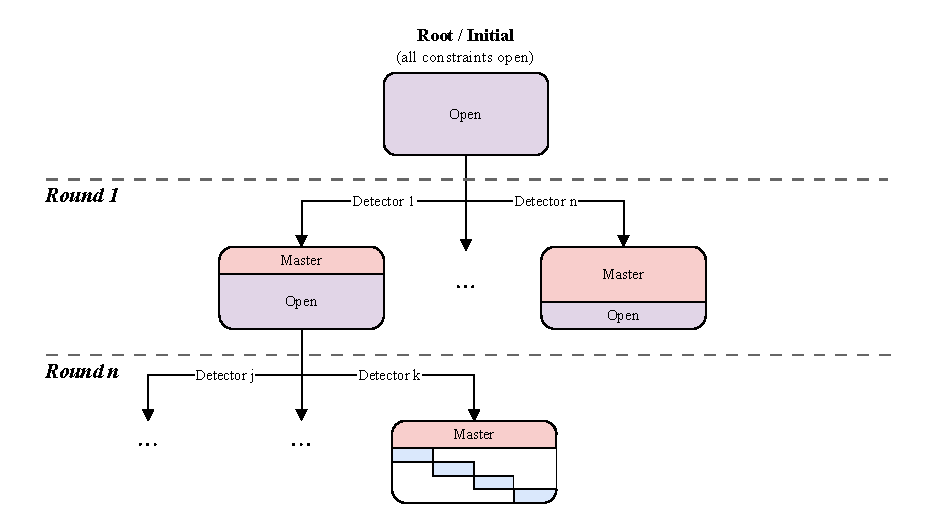
\includegraphics{Bilder/DrawIO/partialdec_tree_pdf}
			\caption{Visualization of the induced tree of propagated partial decompositions.}
			\label{fig:gcg:partialdettree}
		\end{figure}
		
		The concept of detecting structures in different rounds is visualized in Figure \ref{fig:gcg:partialdettree}.
		Starting from a root decomposition in which all constraints are still unassigned or \enquote{open}, different detectors produce a set of new partial decomposition.
		Depending on the configuration, a detector is not allowed to work on a certain partial decomposition or its decedents twice.
		A very simple but concrete example of how such a tree might look like in practice can be found in Section \ref{chap:gcg:example}.
		
		Furthermore, if no detector found any new decomposition in round $k$, or $k$ exceed the maximum number of rounds, the detection loop is stopped and all complete decomposition are collected, scored and exactly one is chosen for which the solving is started. \todo{Grammatik, Wortwahl}
		The scoring and selection stage is of particular interest in practice, because the tree in Figure \ref{fig:gcg:partialdettree} might grow beyond thousand of decompositions, of which the best in terms of solving time or a different metric must be selected.
		Because the scoring of decompositions is not of major interest for \textit{this} thesis, we refer to the official documentation for details \cite{GCG}.
	
	\clearpage
	
	\section{Classifiers}
	\label{chap:gcg:classifiers}
		% 1 Seite, Var Classifiers
		% 1 Seite, Cons Classifiers

		As mentioned in the introduction to this chapter, classifiers are responsible for detecting different underlying structures of the constraint matrix, which can be used during the detection loop to make more informed decisions about which constraints to assign to which block or master.
		Given a set of constraints $C = \{ c_1, c_2, \ldots, c_m \}$, classifiers can be seen as a \textit{injective} function $f: C \mapsto \mathbb{Z}$, i.e., a function that assigns each constraint to exactly one number or \textit{class}.
		Note that in \acs{GCG}, classifiers are allowed to only classify a subset $C' \subseteq C$, leaving $C \setminus C'$ unassigned to any class \footnote{When using \ac{GCG} as a library, this can be checked via. \lstinline|IndexPartition::isIndexClassified|.}.
		In the current version of \ac{GCG}, however, all classifiers always assign every constraint to some class.
		
		Furthermore, each classifier is identified with an unique \textit{name} and an integral priority, influencing the order in which the classifiers are being executed by the framework. 
		
		\subsection{Name Classifiers}
		\label{chap:gcg:classifiers:name}
		
			The names of constraints and variables are, if provided, a strong indicator to which constraints or variables are related to each other.
			The names usually consist of two parts:
			\begin{enumerate}
				\item The semantic group name, such as \enquote{capacity} or \enquote{link} for e.g. a Bin-Packing model. 
				\item A \textit{modifier}, which usually consists of numbers, capital letters or a combination of both. Typically, the modifier is separated from the semantic group name via.  non alpha-numeric characters such as \enquote{\_} or \enquote{\#}.
			\end{enumerate}
		
			Constraints in the same group typically share similar names, with the \textit{modifier} being the only differentiating factor. For example, in a Bin-Packing problem, capacity constraints such as \enquote{capacity\_1}, \enquote{capacity\_2}, $\ldots$ usually vary only in the index indicating the bin. This similarity can be quantified using metrics like the \textit{Levenshtein Distance}, which is the minimum number of single-character edits required to change one word into the other.
			
			\clearpage
			
			Because there is no standardized naming scheme for either variables or constraints, name classifiers usually operate under the assumption that the modeler provided \textit{reasonable} names, if any at all.
			A non-exhaustive collection of different naming schemes observed is provided in Appendix \todo{Appendix}.
			If the modelers provided no names of it's own, then the underlying solver usually chooses a default prefix such as \enquote{c} or \enquote{cons} for constraints, followed by an increasing number, resulting in constraint names \enquote{c0} - \enquote{c4999} for a model with 5000 constraints.
			
			Given a alphabet $\Sigma$, words $w, v \in \Sigma^*$, then the \textit{Levenshtein} distance between those two words can be computed as:
			%
			\begin{equation}
				\label{eq:gcg:levenshtein}
				\mathrm{lev}(w, v) = \begin{cases}
					|w| & \mathrm{if} \; v = \epsilon \\
					|v| & \mathrm{if} \; w = \epsilon \\
					\mathrm{lev}(\mathrm{prefix}(w), \mathrm{prefix}(v)) & \mathrm{if} \; \mathrm{head}(w) = \mathrm{head}(v) \\
					1 + \min \begin{cases}
						\mathrm{lev}(\mathrm{prefix}(w), v) \\
						\mathrm{lev}(w, \mathrm{prefix}(v)) \\
						\mathrm{lev}(\mathrm{prefix}(w), \mathrm{prefix}(v)) \\
					\end{cases} & \mathrm{otherwise}
				\end{cases}
			\end{equation}
			%
			Equation \ref{eq:gcg:levenshtein} can be computed in $O(|w| \cdot |v|)$ using a dynamic programming approach.
			Let $B = (\mathrm{lev}(\mathrm{name}(c_i), \mathrm{name}(c_j)))_{1 \leq i,j \leq m}$ the pair-wise Levenshtein Distance between constraint names, $k \in \mathbb{N}$ the \textit{connectivity} and $G = (V, E)$ with $V = \{ c_1, c_2, \ldots, c_m \}, E = \{ \{ u, v \} \mid u, v \in V, u \neq v, \mathrm{lev}(\mathrm{name}(u), \mathrm{name}(v)) \leq k \}$.
			Furthermore, let $reach(v)$ be the set of reachable vertices from vertex $v \in V$ which is defined as the fix-point of the following function for $s = v$:
			%
			\begin{equation*}
				{reachEventually}_t(T) = \{ u \in V \mid \exists v \in T: v \in E(u) \;  \} \cup \{ t \}
			\end{equation*}
			\todo{WIP}
			%
			Then two constraints $c_i, c_j \in V$ are in the same class iff $c_j \in reach(c_i)$.
			A small example of this concept is shown in Figure \ref{fig:gcg:levenshtein}.
			\todo{5000 cons limit}
			This idea can also be applied to variable names.
			
			\begin{figure}[ht!]
				\centering
				\includesvg[scale=0.8]{Bilder/DrawIO/levenshtein}
				\caption{The graph of pair-wise Levenshtein weights for three capacity constraints. For $k=1$, the edge between $capacity_3$ and $capacity_{12}$ vanishes, but because they is still a connecting path via. $capacity_1$, both constraints are assigned to the same class.}
				\label{fig:gcg:levenshtein}
			\end{figure}
			
			\FloatBarrier
		
		\subsection{Numeric Classifiers}
			
			\subsubsection{Nonzero}
			
				\begin{figure}[ht!]
					\centering
					\begin{equation*}
						A \; = \; \begin{pNiceMatrix}[first-row,first-col,last-col]
							& x_1 & x_2 & x_3 & x_4 & \; \textcolor{red}{class} \\
							{cons}_1 \; & 1 & 5 & -1 & -1 & \quad \textcolor{red}{4} \\
							{cons}_2 \; & 20 & 0 & 0 & 20 & \quad \textcolor{red}{2} \\
							{cons}_3 \;& 20 & 10 & 10 & 0 & \quad \textcolor{red}{3} \\
							{cons}_4 \; & 0 & 100 & -100 & 100 & \quad \textcolor{red}{3} \\
						\end{pNiceMatrix}
					\end{equation*}
					\caption{A constraint matrix with coefficients for each variable. Each constraint is assigned to a class corresponding to its number of non-zero entries.}
					\label{fig:gcg:nonzero}
				\end{figure}
				
				The nonzero classifier classified constraints according to their number of non-zero variable coefficients as shown in Figure \ref{fig:gcg:nonzero}.
				Many types of models including Bin-Packing and Cutting-Stock consist only of constraint groups with a rather \enquote{stable} internal structure, i.e., the capacity constraint for each bin in model \ref{eq:gcg:example:capacity} \todo{Wrong ref} consist of the same number of variables, because each constraint is just a sum over all items differing only in index for the respective bin.
				In general, constraint groups that are suited for this type of classifiers usually involve summations over fixed-sized sets (e.g. a set of items or bins) whose choice is not dependent on any quantified variable.
				Example for the latter include problems whose formulation is based on graphs and usually contains flow-conservation constraints shown in Equation \ref{eq:gcg:numerics:flow}. 
				%
				\begin{equation}
					\label{eq:gcg:numerics:flow}
					\sum_{u \in E(v)} x_{uv} - \sum_{u \in E^{-1}(v)} x_{vu} = 0\quad \forall v \in V
				\end{equation}
				%
				The amount of non-zeros in these constraint is entirely dependent on the number of outgoing and incoming edges for each vertex.
		
			\subsubsection{Objective Function}
			
				A simple classification for variables can be done using information from the objective function, such as:
				
				\begin{enumerate}
					\item Partition variables according to the sign of their coefficient in the objective function. This approach yields three classes in total Positive, Negative and Zero.
					\item Partition them according to the actual \textit{value} of the coefficient.
				\end{enumerate}
				
				Partitioning variables according to the first approach is sufficient for models such as Bin-Packing, in which only the $y$-variables appear in the objective function.
				
				The second approach might partition the variables in too many small cells when e.g. different costs are associated with variables in the objective function.
				This behavior can be observed on model types such as Multi-Commodity-Flow and Unit-Commitment.
				
				\clearpage
		
		\subsection{Type Classifiers}
		\label{chap:gcg:classifiers:type}
		
			Type classifiers examine the constraint matrix to infer a higher-level \textit{type} for each individual constraint.
			A key objective of such classifiers is ensuring or at least improving \textit{robustness}.
			Even minor modifications to a single constraint - such as the removal of one variable - can lead to a different classification, as seen with the previously discussed nonzero classifier.
			Moreover, the likelihood of such changes increases when pre-processing is enabled.
			
			\subsubsection{SCIP Types}
			
				When using \ac{GCG} as a library, the type of a variable or constraint can be retrieved via. \lstinline|SCIPconsGetType(cons)| or \lstinline|SCIPvarGetType(cons)| respectively.
				The former function is not provided by \ac{SCIP} itself, but is implemented in \ac{GCG} instead.
				The implementation compares the name of the handler the constraint is assigned to and compares it to a known list of constraint handlers. \todo{the}
				The list of supported handlers includes \emph{Knapsack}, \emph{Set Partitioning}, \emph{Set Covering}, \emph{Set Packing}, \emph{Varbound} and \emph{General}, in case no special structure was detected. \todo{Check List}
				Variables can be classified as \emph{Integer}, \emph{Binary} or \emph{Continuous}
				\footnote{There are more types of variables in newer versions of \ac{SCIP} such as \emph{Implicit Integer}, but these three basic types are sufficient for the purpose of this discussion.}.
				
				The clear downside of this classification is its important precondition.
				In order to use this feature properly and retrieve a meaningful type via. the two methods, pre-solving must have been executed prior to detection.
				When \ac{GCG} reads the problem as e.g. an \lstinline|.lp| file, all constraints are added as linear constraints to the underlying \ac{SCIP} model.
				These constraints are usually \enquote{upgraded} if possible, that is, their structure is analyzed and assigned to the correct constraint handler during pre-solving.
				This is done in order to take advantage of properties only possessed by certain types of constraints, e.g. a solution to a set of Knapsack constraints \textit{can} be computed more efficiently by using an algorithm based on dynamic programming.
				For more detailed information we refer to the official documentation \cite{SCIPDoxygenDocumentation}.
				Preliminary testing showed that it is not trivial to configure the pre-processing in such a way that \textit{only} the upgrade mechanism is triggered and variables and constraints remain unchanged. \todo{Add test config to appendix}
		
			\subsubsection{MIPLIB Constraint Types}
			
				\begin{table}[ht!]
					\centering
					\begin{tabular}{l|l|l|l}
						\textbf{Nr.} & \textbf{Type} & \textbf{Linear Constraint} & \textbf{Notes} \\
						\hline
						\hline
						1 & Empty & $\emptyset$ & - \\
						2 & Free & $-\infty \leq x \leq \infty$ & No finite side. \\
						3 & Singleton & $a \leq x \leq b$ & - \\
						4 & Aggregation & $ax + by = c$ & - \\
						5 & Precedence & $ax - ay \leq b$ & $x$, $y$ have same type. \\
						6 & Variable Bound & $ax + by \leq c$ & $x \in \{0, 1\}$ \\
						7 & Set Partitioning & $\sum 1 x_i = 1$ & $\forall i: x_i \in \{0, 1\}$ \\
						8 & Set Packing & $\sum 1 x_i \leq 1$ & $\forall i: x_i \in \{0, 1\}$ \\
						9 & Set Covering & $\sum 1 x_i \geq 1$ & $\forall i: x_i \in \{0, 1\}$ \\
						10 & Cardinality & $\sum 1 x_i = b$ & $\forall i: x_i \in \{0, 1\}, b \in \mathbb{N}_{\geq 2}$ \\
						11 & Invariant Knapsack & $\sum 1 x_i \leq b$ & $\forall i: x_i \in \{0, 1\}, b \in \mathbb{N}_{\geq 2}$ \\
						12 & Equation Knapsack & $\sum a_i x_i = 1$ & $\forall i: x_i \in \{0, 1\}, b \in \mathbb{N}_{\geq 2}$ \\
						13 & Bin Packing & $\sum a_i x_i + ay \leq a$ & $\forall i: x_i, y \in \{0, 1\}, b \in \mathbb{N}_{\geq 2}$ \\
						14 & Knapsack & $\sum a_i x_i \leq b$ & $\forall i: x_i \in \{0, 1\}, b \in \mathbb{N}_{\geq 2}$ \\
						15 & Integer Knapsack & $\sum a_i x_i \leq b$ & $\forall i: x_i \in \mathbb{Z}, b \in \mathbb{N}$ \\
						16 & Mixed Binary & $\sum a_i x_i + \sum p_j s_j \; \{\leq, =\} \; b$ & $\forall i: x_i \in \{0, 1\}, \forall j: s_j \; \mathrm{continuous}$ \\
						17 & General Linear & $\sum a_i x_i \; \{\leq, \geq, =\} \; b$ & No special structure.
					\end{tabular}
					\caption{The structure of all 17 constraint types MIPLIB keeps track of.}
					\label{table:constypes:miplib}
				\end{table}
				
				In contrast to the automatic constraint classification performed by SCIP during presolving, the MIPLIB benchmark set provides its own static classification scheme \cite{gleixnerMIPLIB2017Datadriven2021a}. This classification assigns constraints to a set of well-defined structural types such as knapsack, set-partitioning and others as shown in Table \ref{table:constypes:miplib}. Since it is based solely on the syntactic form of the constraints in the original model, it can be applied \textit{independently} of solver presolving.
				Because all types shown in Table \ref{table:constypes:miplib} are deducible only from \textit{local} information such as type of variables and right hand side coefficient, the types can be detected with one pass over the constraint matrix.
				
				This type of classifier shares some issues related to robustness with numeric classifiers.
				Constraint types such as Singleton, Aggregation or Variable Bound depend on the number of non-zeroes, leading to potential miss-classifications on graph based models.
				Furthermore, the only differentiating factor for more \enquote{complex} types such as \textit{Bin Packing} and \textit{Knapsack} is the presence of a variable which happens to have the same coefficient as the right-hand of that constraint.
				
				
	
				\clearpage
	
	\section{Existing Detectors}
	% 1 Seite, trivial Detectors
	% 1 Seite, HMETIS Detectors
	% 1 Seite , other Detectors
	
		\clearpage
	
	\section{Example}
	\label{chap:gcg:example}
		
				\begin{figure}[ht!]
			\centering
			\begin{align}
				&\min &\sum_{j=1}^m y_j \nonumber \\
				&\text{s.t.} &\sum_{j=1}^m x_{ij} &= 1 &&\forall i \in \mathcal{I} \label{eq:gcg:example:link} \\
				&& \sum_{i=1}^n a_i x_{ij} &\leq C y_j && \forall j \in \mathcal{J} \label{eq:gcg:example:capacity} \\
				&& x_{ij} &\in { 0, 1 } && \forall i \in \mathcal{I}, \forall j \in \mathcal{J} \nonumber \\
				&& y_j &\in { 0, 1 } && \forall j \in \mathcal{J} \nonumber
			\end{align}
			\caption{Bin-Packing Model with items $\mathcal{I} = \{ 1, \ldots, n \}$, item sizes $a_i \in \mathbb{Z}_{\geq 0}$, bins $\mathcal{J} = \{ 1, \ldots, m \}$ and capacity $C$.}
			\label{figure:gcg:example:binpack}
		\end{figure}
		\todo{Bild}
		
		\begin{table}[ht!]
			\centering
			\begin{tabular}{l|l|l}
				\textbf{Nr.} & \textbf{Master} & \textbf{Open} \\
				\toprule
				\toprule
				1 & (\ref{eq:gcg:example:link}) & (\ref{eq:gcg:example:capacity}) \\ 
				2 & (\ref{eq:gcg:example:capacity}) & (\ref{eq:gcg:example:link}) \\
				3 & (\ref{eq:gcg:example:link}), (\ref{eq:gcg:example:capacity}) & -
			\end{tabular}
			\caption{For each classifier, the \textit{cons class} detector will produce $2^k - 1$ new partial decompositions with $k$ being the number of classes.}
			\label{table:gcg:example:consclass}
		\end{table}
		
		In order to illustrate the detection with a concrete example, we revisit the textbook Bin-Packing model shown in Figure \ref{figure:gcg:example:binpack}.
		Constraints \ref{eq:gcg:example:link} enforce that every item is packed in exactly one bin, while inequalities \ref{eq:gcg:example:link} ensure that the capacity of each bin is respected if some item is packed in it.
		The objective is to minimize the number of bins.
		
		Without pre-solving enabled, a classifier such as MIPLIB would assign constraints \ref{eq:gcg:example:link} and \ref{eq:gcg:example:capacity} to the classes \textit{Set Partitioning} and \textit{Bin-Packing} respectively.
		If unique, this classification is added to a list provided to the detection stage.
		
		If no further classifications are found, the \textit{cons class} detector will yield 3 new partial decompositions as shown in Table \ref{table:gcg:example:consclass}, first assigning constraints \ref{eq:gcg:example:link}, then \ref{eq:gcg:example:capacity} and finally both \ref{eq:gcg:example:link} and \ref{eq:gcg:example:capacity} to the master.
		The constraint group not assigned to the master remains \textit{open}.
		
		During the next round of detection, a detector such as \textit{Connected Base} will receive the partial decomposition with only the packing constraints assigned to the master as input.
		Here, the induced constraint adjacency graph of the $q \ge 0$ open capacity constraints consists of $q$ isolated connected components, forming the desired block-diagonal structure.
		This process is illustrated in Figure \ref{fig:gcg:example:consclass}.
		
		\begin{figure}[ht!]
			\centering
			\includegraphics{Bilder/DrawIO/example_tree}
			\caption{text}
			\label{fig:gcg:example:consclass}
		\end{figure}
		
\chapter{Tree Refinement}
\label{chap:tree}
% 0.5 Seiten

	With the existing capabilities of \ac{GCG} presented in the previous chapter, we continue with the main contributions of this thesis:

	\begin{itemize}
		\item A new module which is integrated into the detection framework of \ac{GCG} for reverse engineering semantic groupings of the original formulation. This can be seen as a generalization of the approach presented in \cite{salvagninDetectingSemanticGroups2016}
		\item Additional auxiliary classifiers which implement constraint and variable classification based on information not currently used including examples of \textit{when} they are crucial detecting semantics.
	\end{itemize}

	This chapter is divided into three main section:

	\begin{enumerate}
		\item A short summary about the available information we have access to.
		\item What the motivation and goals are why and how we aim to process this information.
		\item The concrete algorithm and its most integral parts.
	\end{enumerate}

	Some concrete details about the implementation itself are not subject of the following sections, but are discussed in Chapter \ref{chap:impl}.

	\clearpage

	\section{The Algorithm}
	% 2 Seiten

		In \cite{salvagninDetectingSemanticGroups2016}, the implemented approaches can be seen as a three-step process:

		\begin{enumerate}
			\item Transform a given model to a graph-based representation.
			\item Select a suitable initial partitioning.
			\item Choose \textit{one} splitter-function and run the standard partition refinement algorithm until a stable partition is reached.
		\end{enumerate}

		Depending on the type of model, running the refinement with different initial partitions and splitter-functions might be necessary, which was already recognized in \cite{salvagninDetectingSemanticGroups2016}.
		Furthermore, we suspect that for some models it might even be required to use different splitter-funtions on different \textit{parts} of the model.

		In the following, we will generalize this process by adopting a similar approach as the one shown in Chapter \ref{chap:gcg}.
		Instead of choosing \textit{one} way of refining the constraints or variables based on an initial partition, we try different \textit{strategies} to explore a more broader search space.
		Afterwards, the found partitions are scored using a family of scoring functions $g_i: \Pi(U) \rightarrow \mathbb{R}$ and the most promising ones are selected.
		Note that the overall goal remains unchanged: Based on an initial partition, we aim to iteratively refine the cells in such a way, that ultimately the constraints or variables in each cell belong to the same semantic grouping as the modeler intended to.

		In order to achieve this, we propose multiple \textit{strategies} which form the basic building blocks of the algorithm and are discussed in Section \ref{chap:tree:strategies}.
		Each strategy takes a single cell $C_i$ as input and computes a partition $\pi_{C_i} \in \Pi(C_i)$ as output, thereby refining the cell.
		In the following, the process of refining a cell according to a certain strategy is sometimes referred to as \enquote{expanding a cell}.
		The partitions of the cells are organized in a \acf{SRT} as shown in Figure \ref{fig:tree:motivation}, i.e., each node, with exception of the root node, corresponds to a possible partitioning of its parent cell, which was computed by a strategy.
		The root node and its cells correspond to the initial partition and it is the \textit{only} node for which the union of its cells corresponds to the whole set of constraints or variables. The cells of all other nodes only partition its immediate parent cell in the tree.
		This process implies that an additional post-processing step is required which translates the tree of cell-refinements to actual partitions. This step is discussed in Section \ref{chap:gcg:scoring}.

		\begin{algorithm}
			\centering
			\begin{algorithmic}
				\Require Initial partition $\pi_{\mathrm{init}}$, set of strategies $S = \{ f_1, f_2, \ldots, f_k \}$ with $f_i: P \mapsto \Pi(P)$
				\Ensure List of partition $\Pi$
				\Statex
				\Function{TreeRefinement}{$\pi_{\mathrm{init}}$}
					\State Init empty \ac{SRT} $T = \srt$
					\State $queue \gets \text{Create queue with element} \; \pi_{\mathrm{init}}$
					\While{\Call{Size}{$queue$} $\ge 0$}
						\State $\pi_{\mathrm{current}} \gets$ \Call{Pop}{$queue$}
						\For{$cell \in \pi_{\mathrm{current}}$}
							\For{$f_{\mathrm{strategy}} \in S$}
								\State $refined \gets f_{\mathrm{strategy}}(\pi_{\mathrm{current}})$ \Comment{Section \ref{chap:tree:strategies}}
								\State \Call{Push}{queue, refined}
							\EndFor
						\EndFor
					\EndWhile

				\EndFunction
			\end{algorithmic}
			\caption{A high-level overview of the algorithm. All additional data structures, optimizations and handling of necessary metadata was omitted.}
			\label{fig:tree:algo}
		\end{algorithm}
		\todo{WIP}

		In order to use a unified notation in the following sections, we will define the \ac{SRT} and its associated information more formally.
		A \ac{SRT} can be formalized as a tuple $T = (V, E, U, R, S)$ with universe $U$ corresponding to the set of all constraints or variables, designated root node $R \in V$ and set of strategies $S \subseteq \mathbb{N}$.
		The tuple $(V, E)$ must induce an directed acyclic graph.
		Each node $v \in V \setminus R$ of the tree is associated with a parent cell $\mathrm{ParentCell}_v \in 2^U$, parent node $\mathrm{ParentNode}_v$, a set of cells $\mathrm{Cells}_{v} \in \Pi(\mathrm{ParentCell}_v)$ and the strategy $\mathrm{Strategy}_v$ that was used to compute $v$ from its parent.
		For the root node it holds that $\mathrm{Cells}_R \in \Pi(U)$.

		\begin{figure}[ht!]
			\centering
			\includesvg[scale=0.5, inkscapelatex=false]{Bilder/Hierarchy/hierarchy_binpack_NOP}
			\caption{WIP WIP WIP A example of a simple refinement tree for the Bin-Packing Problem.}
			\label{fig:tree:motivation}
		\end{figure}
		\todo{wrong image}

		\clearpage

	\section{Information}
	% 1 Seite

		\begin{figure}[ht!]
			\centering
			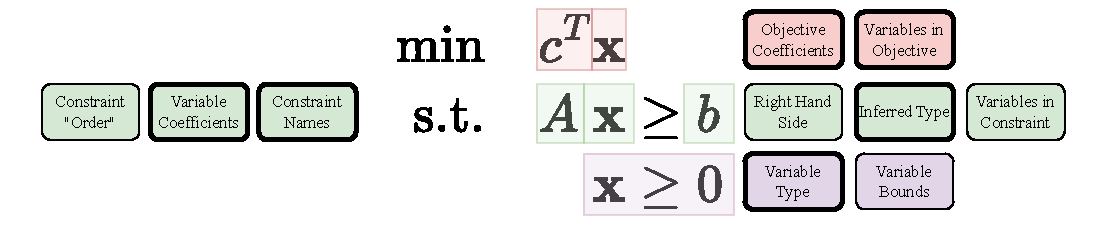
\includegraphics[scale=0.8]{Bilder/DrawIO/model_information}
			\caption{All parts of a model that contain useful information for semantic grouping of constraints and variables. Elements with a thick border are already used as a key concept in one of the existing detectors.}
			\label{fig:tree:information}
		\end{figure}

		Before we present any algorithmic details, we give an overview about the available information which might be used to define suitable strategies. \todo{roter Faden}

		\begin{enumerate}
			\item \textbf{Objective}: For the objective functions, information about the participating variables and their coefficients is available. For some models e.g. for Bin-Packing, this information alone is sufficient to partition the variables.
			\item \textbf{Coefficients}:
			The use of coefficients to classify constraints and variables was already in discussed in Section \ref{chap:gcg:classifiers}.
			\item \textbf{Bounds}: For all variables $lb \leq x \leq ub$ information about their lower- and upper-bounds is available.
			Furthermore, the left- and right-hand-side of linear constraints $lhs \leq \sum_i a_i x_i \leq rhs$ are available as well.
			\item \textbf{Types}: Variable types such as \textit{Integer} are usually stated explicitly in the input format. If not, then information about the variable bounds can be used to deduce a type, e.g. $0 \leq x \leq 1$ is a strong indicator that $x$ is a \textit{Binary} variable.
			\item \textbf{Names}: If specified by the modeler, then variables and constraints might have meaningful names which can be used as a strong indicator which constraints and variables belong to the same group.
			\item \textbf{Order}: In contrast to other kinds of information, the constraint \enquote{order} is no intrinsic property of the model itself. With the term \enquote{order}, we refer to the order of the constraints as specified in the input format. When a model is created e.g. via. a script, constraints are usually added in \textit{blocks} by the modeler. This information is used in Section \ref{chap:tree:classifiers:voting} to conceptualize a classifier based on that.
		\end{enumerate}

	\section{Classifiers}
	% 2 Seite

		In the following Sections we describe different classifiers which are not yet implemented in \ac{GCG} but could potentially provide new information about the model.
		Adding new classifiers has, in addition to practical implications such as higher maintenance overhead, additional side-effects regarding runtime and memory requirements.
		Each new classifier provides new opportunities for existing detectors to find new partial decompositions.
		This can prove especially useful for detectors like consclass, which directly depend on the found classifications.
		On the other hand, this dependence can result in a sub-optimal runtime investment if the found classifications provide no new information, because the generated partial decompositions based on that will most certainly be of bad quality as well. \todo{wording}
		Therefore, we will refrain from mentioning all missing model properties for which a classifier \textit{could} be built, and only focus on promising candidates.
		\todo{Summarize goals for custom classifiers}

		\subsection{Bounds}

			When considering bounds, we differentiate between variables and constraint respectively.

			\subsubsection{Variable bounds}

				The classifier for variable bounds can be considered as a simple mapping from pairs of bounds to a unique class index.
				More formally, given a list of all unique pairs of lower and upper bounds for variables $B = (b_1, b_2, \ldots, b_k)$, with $b_i \in \mathbb{Q} \times \mathbb{Q}$, we map each variable to the index of its bounds in $B$.
				This mapping is trivially unique.

				Mapping the variables in the described way has the side-effect that $0 \leq x \leq 1$ and $y \in \{ 0, 1 \} $ are mapped to the same class.
				This behavior is able to account for missing declarations of variables as binary in the input format read by \ac{GCG}.
				The classification is wrong if $x$ is truly meant to be a continuous variable, but this is offset by the fact that \ac{GCG} already includes a classifiers based on \ac{SCIP} types, which will correctly classify both variables in this case.

				Types of models where information about the variable bounds \textit{can} be leveraged include instances of e.g. Container Loading.
				Here, variables $x, y, z \in \mathbb{R}$ encoding the positions of parcels to be loaded into a container are continuous. If the container is not a cube, i.e., it has a different length in each spacial dimension, then the variables have to have different bounds.

			\subsubsection{Constraint bounds}

				A classifier for constraint bounds works in a similar manner as for variables.
				By collecting all bounds and assigning a class to each constraint based on that list, we obtain a unique mapping.
				Note that for inequalities the absolute value either of the two bounds will always be infinity. For equalities which were not replaced with equivalent inequalities, both bounds will be equal.

				In addition to a classifier based on the actual \textit{values} of the bounds, i.e., for values $a, b \in \mathbb{R}$ of a linear constraint $a \leq \sum a_i x_i \leq b$, we propose a classifier based on the \textit{sign} of  $a$ and $b$.
				Here, the linear constraint is transformed to standard form to prevent a different classification for equivalent constraints in case the constraint is multiplied by $-1$.
				Therefore, only four potential classes shown in Table \ref{table:tree:classifiers:bounds:exist} remain.
				This classifier can be used for variables analogously.

				\begin{table}[ht!]
					\centering
					\begin{tabular}{l|l|l|l}
						\textbf{Class Nr.} & \textbf{Name} & \textbf{$sign(a)$} & \textbf{$sign(b)$} \\
						\toprule
						\toprule
						1 & Positive & $+$ & $+$ \\
						2 & Mixed &$+$ & $-$ \\
						2 & Mixed & $-$ & $+$ \\
						3 & Negative & $-$ & $-$ \\
						4 & Zero $(a = b = 0)$ & $+/-$ & $+/-$
					\end{tabular}
					 \caption{The four classes of the sign-variant of the bounds classifier.}
					 \label{table:tree:classifiers:bounds:exist}
				\end{table}

				\todo{cap. lot sizing example}

				\clearpage

		\subsection{Relaxed MIPLIB types}

				\begin{table}[ht!]
				\centering
				\begin{tabular}{l|l|l|l}
					\textbf{Nr.} & \textbf{Type} & \textbf{Linear Constraint} & \textbf{Notes} \\
					\hline
					\hline
					1 & Empty & $\emptyset$ & - \\
					2 & Free & $-\infty \leq x \leq \infty$ & No finite side. \\
					3 & Singleton & $a \leq x \leq b$ & - \\
					4 & Aggregation & $ax + by = c$ & - \\
					5 & Precedence & $ax - ay \leq b$ & $x$, $y$ have same type. \\
					6 & Variable Bound & $ax + by \leq c$ & $x \in \{0, 1\}$ \\
					7 & Set Partitioning & $\sum 1 x_i = 1$ & $\forall i: x_i \in \{0, 1\}$ \\
					8 & Set Packing & $\sum 1 x_i \leq 1$ & $\forall i: x_i \in \{0, 1\}$ \\
					9 & Set Covering & $\sum 1 x_i \geq 1$ & $\forall i: x_i \in \{0, 1\}$ \\
					10 & Cardinality & $\sum 1 x_i = b$ & $\forall i: x_i \in \{0, 1\}, b \in \mathbb{N}_{\geq 2}$ \\
					11 & Invariant Knapsack & $\sum 1 x_i \leq b$ & $\forall i: x_i \in \{0, 1\}, b \in \mathbb{N}_{\geq 2}$ \\
					12 & Equation Knapsack & $\sum a_i x_i = 1$ & $\forall i: x_i \in \{0, 1\}, b \in \mathbb{N}_{\geq 2}$ \\
					13 & Bin Packing & $\sum a_i x_i + ay \leq a$ & $\forall i: x_i, y \in \{0, 1\}, b \in \mathbb{N}_{\geq 2}$ \\
					14 & Knapsack & $\sum a_i x_i \leq b$ & $\forall i: x_i \in \{0, 1\}, b \in \mathbb{N}_{\geq 2}$ \\
					15 & Integer Knapsack & $\sum a_i x_i \leq b$ & $\forall i: x_i \in \mathbb{Z}, b \in \mathbb{N}$ \\
					16 & Mixed Binary & $\sum a_i x_i + \sum p_j s_j \; \{\leq, =\} \; b$ & $\forall i: x_i \in \{0, 1\}, \forall j: s_j \; \mathrm{continuous}$ \\
					17 & General Linear & $\sum a_i x_i \; \{\leq, \geq, =\} \; b$ & No special structure.
				\end{tabular}
				\caption{The structure of all constraint types which the \textit{relaxed} version of the MIPLIB classifier detects.}
				\label{table:constypes:relaxed}
			\end{table}

			In order to mitigate \textit{some} of the issues

			Similar to the MIPLIB classifier, all types can be deduced from local information only. Thus, one pass over the constraint matrix is sufficient to classify all constraints according to Table \ref{table:constypes:relaxed}. \todo{WIP}

			\clearpage

		\subsection{Voting}
		\label{chap:tree:classifiers:voting}

			As mentioned earlier, the motivating idea behind each individual classifier is to group constraints according to some property, while the type of this property can vary greatly between classifiers.
			Under the assumptions that groups of constraints share at least \textit{some} of these properties and are thus assigned to the same classes, we can define a new type of classifier.
			Note that this classifier can be equivalently conceptualized as an additional \textit{strategy}, which are the basic building blocks of the refinement algorithm and explained in Section \ref{chap:tree:strategies}.
			This assumption is, at least on examples that can be observed in practice, a reasonable one.

			\subsubsection{Voting (unordered)}

				\begin{figure}[ht!]
					\centering
					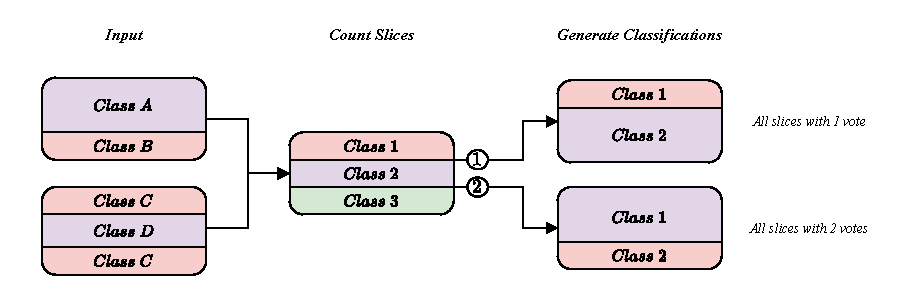
\includegraphics[scale=1.05]{Bilder/DrawIO/strat_ordered_voting_pdf}
					\caption{text}
					\label{fig:tree:classifiers:ovoting}
				\end{figure}

				In order to derive a simple and efficient algorithmic approach to this problem, we can make an additional assumptions not based on the model itself, but on its representation in common input formats like \lstinline|.lp| and \lstinline|.mps| files.
				A lot of models are generated via. scripts and written to such files for portability and interoperability with other solvers.
				One exploitable property which can be observed in a lot of models is, that groups constraints are usually \textit{added in bulk}.
				This results in consecutive blocks of constraints which are semantically related, which is illustrated in the \enquote{Input} column of Figure \ref{fig:tree:classifiers:ovoting}.
				If a class of constraints is split into two non-consecutive groups like the second partition from Figure \ref{fig:tree:classifiers:ovoting}, then we can deduce that they are meant to be two different groups.

			\subsubsection{Voting (unordered)}
			\label{chap:tree:classifiers:cooccurence}

				If the read model does \textit{not} have the property of properly ordered constraint blocks, a more involved algorithmic approach can be used.
				Here, the general problem can be reduced to group constraints with each other which are \textit{often} assigned to the same class. \todo{WIP}

				\clearpage

%	\section{Tree Refinement}
%	% 4 Seiten
%
%		\begin{figure}[ht!]
%			\centering
%			\includesvg{Bilder/Hierarchy/hierarchy_binpack_NOP}
%			\caption{Test}
%			\label{fig:tree:binpackNOP}
%		\end{figure}

	\section{Strategies}
	\label{chap:tree:strategies}

		Strategies are \textit{the} central building block of the algorithm and are responsible for refining sets of constraints or variables.
		Let $U$ be a the total set of constraints or variables.
		Each strategy can be formalized as a function $f: S \rightarrow \Pi(S)$ which gets a single set $S \subseteq U$ as input and produces a partition $\pi \in \Pi(S)$ as output.
		Conceptually, each strategy can be seen as a materialization of a specific splitter function as defined in Section \ref{chap:prelims:partitionref}.

		%In the following, we differentiate between re-callable and non re-callable strategies. The former type may be called more than once in any given sub-tree, as the result may depend on precise position of the node that is being expanded.

		\subsection{Slice (Partition)}
		\label{chap:tree:strategies:slice:part}

			\begin{figure}[ht!]
				\centering
				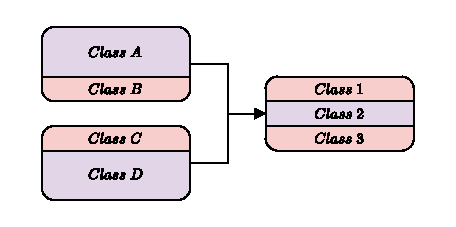
\includegraphics[scale=1.2]{Bilder/DrawIO/strat_slicing_pdf}
				\caption{A simplified illustration assuming that constraint in both partitions can be rearranged into continuous blocks, thus \enquote{slicing} the partitions into different-sized chunks. The output partition inherits all these slices.}
				\label{fig:tree:strat:slice}
			\end{figure}

			Slicing strategies are the most simple type of strategy.
			Given two partition $\pi, \pi' \in \Pi(U)$, we define the \textit{combined partition} $\pi \sqcap \pi'$ as follows:
			%
			\begin{equation}
				\label{eq:tree:strat:slice:overlay}
				\pi \sqcap \pi' = \{ A_i \cap B_j \mid A_i \in \pi, B_j \in \pi' \} \setminus \emptyset
			\end{equation}
			%
			This concept is illustrated in Figure \ref{fig:tree:strat:slice}.
			Because strategies only refine single sets and not whole partitions, Equation \ref{eq:tree:strat:slice:overlay} always degenerates to $\pi_{slice} \sqcap \{ S, U \setminus S \}$ for some partition $\pi_{slice} \in \Pi(U)$ and a set $S$ we want to refine.
			The result is then restricted to elements of $S$, which yields a partition of $S$.
			More formally, this strategy can be expressed as Function \ref{eq:tree:strat:slice:function} and computed efficiently using Algorithm \ref{algo:tree:strat:slice}.
			%
			\begin{equation}
			\label{eq:tree:strat:slice:function}
				f_{\pi_{splitter}}(S) = \left\{ A_i \cap S \mid A_i \in \pi_{splitter} \right\} \setminus \emptyset
			\end{equation}
			%
			Note that the operator $\sqcap$ is trivially associative, i.e., $(\pi \sqcap \pi') \sqcap \pi'' = \pi \sqcap (\pi' \sqcap \pi'')$:
			%
			\begin{alignat*}{4}
				X \in (\pi \sqcap \pi') \sqcap \pi'' &\iff \exists Z \in (\pi \sqcap \pi'), C \in \pi'' && : \; && X && ={} Z \cap C \\
				&\iff \exists A \in \pi, B \in \pi', C \in \pi''&& : \; && X && ={} (A \cap B) \cap C \\
				&\iff \exists A \in \pi, B \in \pi', C \in \pi''&& : \; && X && ={} A \cap (B \cap C) \\
				&\iff  X \in \pi \sqcap (\pi' \sqcap \pi'')
			\end{alignat*}

			In conjunction with commutativity, this fact can be used to e.g. eliminate part of the search space by pruning duplicated nodes in the tree and only expanding one instance of any given sub-tree.

			A simple example where two successive applications of this slicing strategy can

			\begin{algorithm}[ht!]
				\centering
				\begin{algorithmic}
					\Require Partition $\pi = \{ A_1, A_2, \ldots, A_k \}$, set $S \subseteq U$, function $f_C: U \mapsto \mathbb{N}$ for $C = \{ C_1, C_2, \ldots \} \in \Pi(U)$ mapping $u \in U$ to $C_i$ iff $u \in C_i$
					\Ensure Partition of $S$ according to Function \ref{eq:tree:strat:slice:function}.
					\Statex
					%
					\Function{strategySlice}{$\pi, S$}
						\State $\pi_{out} \gets$ list of $k$ empty sets $B_1, B_2, \ldots, B_k$
						\For{$s \in S$}
							\State $i \gets f_S(s)$
							\State $B_i \gets B_i \cup \{ s \}$
						\EndFor
						\State Remove empty sets from $\pi_{out}$
						\State \Return $\pi_{out}$
					\EndFunction
				\end{algorithmic}
				\caption{If a lookup table represented by function $f$ is available, then Function \ref{eq:tree:strat:slice:function} can be implemented in O($|S|$).}
				\label{algo:tree:strat:slice}
			\end{algorithm}

			\FloatBarrier
			\clearpage

		\subsection{Slice (Covering)}

			\begin{figure}[ht!]
				\centering
				\includesvg[scale=1.25]{Bilder/DrawIO/setcov}
				\caption{Given $U = \{ 1, \ldots, 6 \}$, and $S = \{ \{ 1, 2, 3 \}, \{ 3, 4 \}, \{ 4, 5, 6 \} \} \subseteq 2^U$, with each $C \in S$ corresponding to one \textit{feature}.
				Each element $x \in U$ is part of at least one set $C \in S$, thus possessing at least one feature.
				This example can be encoded as a graph, where the right side \enquote{the features} are pre-partitioned into individual cells. By applying the standard partition refinement framework from Section \ref{chap:prelims:partitionref} with function \ref{eq:prelims:pref:exists}, we obtain a partition $\pi \in \Pi(U)$ in which the elements any given cell possess the same features.}
				\label{fig:tree:strat:cov}
			\end{figure}

			%Before we explain the \textit{covering} version of the previous strategy, Function \ref{eq:tree:strat:slice:function} can be seen as an instantiation f
			Let $U$ be an arbitrary set. Then a covering can be defined as a set $S \subseteq 2^U$, where $S^U$ denotes the power set, such that:
			%
			\begin{equation*}
				U = \bigcup_{C \in S} C
			\end{equation*}
			%
			The definition is equivalent to a set partitioning without the condition that sets of $S$ must be pairwise disjuct.
			Each set $C \in S$ corresponds to one \textit{feature}, with the elements $x \in C$ considered to possessing said feature.
			The goal of the covering version of the slicing strategy is to partition the elements of a given set in such a way, that elements in the same cells all possess the same features.
			In order to obtain such a partition from a set covering $S$, we can encode the underlying problem as a graph and use the standard partition refinement framework.
			%The splitter-function that is being used here corresponds to Function \ref{eq:prelims:pref:exists}.
			Afterwards, the resulting partition can be used to slice the given set as described in Section \ref{chap:tree:strategies:slice:part}.

			The strategy can be used to e.g. partition constraints according to the types of variables that they contain.
			It is functionally equivalent to the refinement method \enquote{fast} from \cite{salvagninDetectingSemanticGroups2016}.
			The name most likely stems from an algorithm informally described a fast algorithm based on bucket sort to implement such a partition refinement algorithm. \todo{Example}

			\clearpage

		\subsection{Recursive}

			\begin{figure}[ht!]
				\centering
				\includesvg[scale=1.25]{Bilder/DrawIO/strat_rec}
				\caption{An example of a graph for which the partition refinement algorithm takes multiple iterations to yield a stable partition (Function \ref{eq:prelims:pref:exists}). Red circles around the vertices highlight changes to the cells in the respective iterations. The algorithm is initialized with $\pi_{init} = \{ \{ 1, 2 \}, \{ 3, 4 \}, \{ A, B, C, D \} \}$. During the first iteration, all vertices on the right side are in the same cell so no changes can happen on the left side. Vertices $A, B$ are not connected to cell $\{ 3, 4 \}$. A similar reasoning applies for the second iteration.}
				\label{fig:tree:strat:rec}
			\end{figure}

			The \textit{recursive} strategy is the the only strategy which needs to utilizes the full blown partition refinement framework.
			The strategy is based on the canonical constraint-variable un-directed graph already shown in Figure \ref{fig:prelims:graphs:binpackbipartite}.
			Each variable and constraint corresponds to exactly one vertex, while an edge between a constraint and variable node exists iff the variable is part of the constraint.
			More formally, given a set of constraints $C = \{ c_1, \ldots, c_m \}$ and a set of variables $X = \{ x_1, \ldots, x_n \}$. Let $a_{ij}$ be the coefficient of variable $x_i \in X$ in constraint $c_j \in C$.
			Then we can define the graph as follows:
			%
			\begin{equation*}
				G = (V, E) = (X \cup C, \{ \{ x_i, c_j \} \mid x_i \in X, c_j \in C, a_{ij} \neq 0 \})
			\end{equation*}
			%
			The size of the graph in terms of it's edges and vertices depends entirely to the underlying problem.
			A partition is obtained by running the algorithm with either Function \ref{eq:prelims:pref:count} or Function \ref{eq:prelims:pref:exists}.
			Afterwards, the partition is used to slice a given set according to the method described in Section \ref{chap:tree:strategies:slice:part}.
			Note that even thought the generated graph is always bi-partite, it does not necessarily fulfill the conditions mentioned in Section \ref{chap:prelims:partitionref} for the fast variant of the refinement algorithm, i.e., that all nodes on one of the two sides of the bi-partite graph are all in their own cell.
			As a consequence, one full execution of the recursive strategy might take orders of magnitude longer than an execution of one of the two slice variants explained previously. \todo{"orders of magnitude" ein wenig übertrieben}

			\clearpage

	\section{Cutoff Conditions}
	\label{chap:impl:cutoff}

		In order to limit the size of the tree and ensure that we only explore relevant parts of the search space, we propose several conditions the terminate the search early on.
		The conditions can be divided into two groups:

		\begin{enumerate}
			\item \textit{Local} Conditions, which can be evaluated by only considering information about one \textit{singular} node or its immediate predecessor.
			\item \textit{Global} Conditions, whose evaluation requires information about e.g. the precise path to the node, i.e., its position in the tree and therefore information about its ancestors, \textit{or} requires knowledge about other nodes or completely distinct sub-trees.
		\end{enumerate}

		Note that the following conditions are only \textit{correct} for the strategies presented in Section \ref{chap:tree:strategies}, which are all a specialized version of the partition slicing strategy.
		In the following, let $T = \srt$ be a \ac{SRT}.

		\subsection{Local Conditions}
		% 1 Seite

			With access only to local information, these conditions are restricted to the information about a single node $v_0 \in V$.

			\subsubsection{Refined Partition Size}

			Assuming a proper ground-truth is available or any heuristic information about the potential size $k \in \mathbb{N}$ of the target partition, many found nodes can be excluded from the scoring a-priori. \todo{WIP}
			We can terminate search for the sub-tree rooted at $v_0$ if $| \mathrm{Cells}_{v_0} | \gg k$.

			\subsubsection{No Changes}

			As soon as the algorithm expands a set $S$ with a strategy, we get a partition $\pi \in \Pi(S)$ as a result.
			If $S \in \pi$, this implies that $\pi = \{ S \}$ and the strategy did not refine $S$ any further and we can terminate the search for the current sub-tree.

		\subsection{Global Conditions}
			% 1 Seite

			As mentioned before, global conditions are more flexible and allow for more involved logic to be executed.

			\subsubsection{Depth}

				Under the assumption that most of the \enquote{interesting} sets are found early on, it could be beneficial to abort the search for a sub-tree as soon as a certain depth has been reached.
				The depth of a certain node $v \in V$ can be computed using a simple recursion to the root node:
				\begin{equation*}
					\mathrm{Depth}(v) = \begin{cases}
						0 & \text{if} \; v = R \\
						1 + \mathrm{Depth}(\mathrm{ParentNode}_v) & \mathrm{otherwise}
					\end{cases}
				\end{equation*}

			\subsubsection{Sub-Tree Duplication}

				If $v_0$ is expanded by the algorithm, then all cells of the node are expanded by all strategies that did not run previously.


			\subsubsection{Most Optimistic Partition Size}

				Similar to the local condition terminating the search at a node $v \in V$ exceeding a certain number $k \in \mathbb{N}$ of cells, we can terminate the search as it becomes evident that the size of \textit{any} partition containing $v$ and is generated by function \ref{eq:tree:scoring:partcomp} will exceed $k$.
				This \textit{Most optimistic partition size}, i.e., the size of the smallest partition that can be generated using $v$, can be computed as shown in Function \ref{eq:tree:cutoff:mos}.
				%
				\begin{equation}
				\label{eq:tree:cutoff:mos}
					\mathrm{MOS}(v) = \begin{cases}
						0 & \text{if} \; v = R \\
						|\mathrm{Cells}_{\mathrm{ParentNode}_v}| + \mathrm{MOS}(\mathrm{ParentNode}_v) - 1 & \mathrm{otherwise}
					\end{cases}
				\end{equation}
				%
				Because all nodes in the \ac{SRT} are non-empty, it trivially holds that $\mathrm{MOS}(v) \geq \mathrm{MOS}(\mathrm{ParentNode}_v)$ for all $v \in V$.
				As soon as $MOS(v) \gg k$, we can terminate the search as all partitions generated using at last one descendant of $v$ will exceed the threshold.

		\subsection{Side effects of global conditions}

			Conditions such as \textit{Depth} or \textit{Most Optimistic Partition Size} can have unintended side-effects in combination with other global conditions like \textit{Sub-Tree Duplication}.


			\begin{figure}[ht!]
				\centering
				\includesvg[scale=0.5, inkscapelatex=false]{Bilder/Hierarchy/hierarchy_binpack_NOP}
				\caption{text}
				\label{fig:tree:cutoff:mos}
			\end{figure}
			\todo{Falsches Bild}

	\clearpage

	\section{Scoring}
	\label{chap:gcg:scoring}
	% 1 Seite

		Up until this point we have only described how the algorithm refines sets based on different strategies, despite the goal being a list of promising partitions.
		Before we describe how to select such partitions, we have to define how we actually \textit{get} a list of partitions from the refinement tree.

		Let $G = (V, R, E)$ the set refinement tree with vertex set $V$, designated root node $R \in V$ and edges $E \subseteq V \times V$. \\
		Let $Recombine_k(U_1, U_2, \ldots, U_k): U_1 \times U_2 \times \ldots \times U_k \xrightarrow{} 2^{U_1 \cup U_2 \cup \ldots \cup U_k}, k \in \mathbb{N}$ be a Function defined as follows:
		%
		\begin{equation*}
			Recombine_k(U_1, U_2, \ldots, U_k) = \begin{cases}
				\emptyset & k = 0 \\
				U_1 & k = 1 \\
				\{ \{ u \} \cup r \mid u \in U_1, r \in Recombine_{k-1}(U_2, U_3, \ldots, U_k) \} & else
			\end{cases}
		\end{equation*}
		%
		More informally, $Reombine_k$ takes a total of $k$ arbitrary sets $U_1, \ldots, U_k$ and computes a set containing all possible $k$-tuples $(u_1, u_2, \ldots, u_k)$ with $u_i$ restricted to elements from $U_i$.
		Thus, the set of \textit{all} partitions constructible from a sub-tree rooted at vertex $v \in V$ can be computed using Function \ref{eq:tree:scoring:partcomp}.
		%
		\begin{equation}
		\label{eq:tree:scoring:partcomp}
			Partitions(v) = \begin{cases}
				Sets(v) & \text{if $v$ is leaf node} \\
				\left\{ Recombine_{|Sets(v)|} \right\} & else
			\end{cases}
		\end{equation}
		\todo{WIP}
		%
		It is clear that setting $v = R$ gives the set of all possible partitions.
		\todo{Add simple proof}

		One can deduce from the definition of Function \ref{eq:tree:scoring:partcomp} that the number of partitions depends on the depth and maximum out-degree of any given node of the tree.
		Therefore, it will be of vital interest to only consider \enquote{interesting} sets.
		Ideas and possible implementations are discusses in Chapter \ref{chap:impl}.

		\clearpage

		\subsubsection{Example}

			\begin{figure}[ht!]
				\centering
				\includesvg[scale=0.5, inkscapelatex=false]{Bilder/Hierarchy/scoring_example}
				\caption{A sample \ac{SRT} with four nodes. Node 1 has one descendant, so the recursive function will generate multiple possible partitions because of that.}
				\label{fig:tree:scoring:example}
			\end{figure}

			In order to illustrate the generation of partition from a given \ac{SRT}, we use the tree shown in Figure \ref{fig:tree:scoring:example} as an example.
			In the following, we abbreviate a node \enquote{Node $i$} with $N_i$.
			Applying the definition of Function \ref{eq:tree:scoring:partcomp} to the \ac{SRT}, we have start at the root node with identifier 0.
			%
			\begin{equation*}
				Partitions(N_0) = {Recombine}_1
			\end{equation*}
			\todo{WIP}
			%
			Because the root node only consists of one cell, we just take the union of $Partitions(N_1)$ and $Partitions(N_3)$.
			For the latter, we can compute the result easily, because $N_3$ is a leaf node. Thus, the set of all possible ways of generating partitions for cell 0 in this sub-tree consists of the single partition $\{ \{ 1, 3, 4 \} \}$
			For $N_1$, we have to execute the recursion twice:

			\begin{enumerate}
				\item The first possibility to partition cell 0 is $\{ 1, 2 \}$.
				\item In addition, we have another option to partition set $2$: $\{ 3, 4 \}$, which is possible because of Node 9.
			\end{enumerate}

			Thus, we can partition cell 0 in this sub-tree in two ways: $\{ \{ 1, 2 \}, \{ 1, 3, 4 \} \}$.
			The union of the left and right sub-tree results in three possible ways to partition cell 0, finishing the partition generation phase.

		\clearpage

		\subsection{Constraint Names}
		\label{chap:tree:scoring:names}

			One important piece of information that usually reflects the modelers \textit{intent} when it comes to the semantic difference are the names of the constraints or variables, in the following abbreviated with just \enquote{names}.
			As discusses in Section \ref{chap:gcg:classifiers:name}, names usually consist of multiple parts, with one part containing all the information related to \textit{semantics}.
			Extracting this part of the name can be done heuristically using Algorithm \ref{algo:tree:scoring:nameheur}.
			The heuristic consist of four major steps:
			\begin{enumerate}
				\item Remove \textit{modifies} which are usually enclosed in either brackets or some other special character combination which consists of an \textit{opening} and \textit{closing} character.
				\item \enquote{Normalize} the string by replacing any non-alpha-numeric separators such as spaces, tabs, $\ldots$ with a single character $c$ such as \enquote{\_}.
				\item Split the string according to $c$ and try to detect the part with the relevant semantics.
				\item \textit{(Optional)} Remove any left-over non-alpha characters such as numbers.
			\end{enumerate}

			Step 4 is explicitly marked as optional, because sometimes numbers are integral part of the name, sometimes they are not.
			Both of these cases can actually be observed in the same model \footnote{StrIPlib UUID: d48c9568-e0ea-4c77-9a3b-b7f4dc530d5f}.
			For this model in particular, the constraints \enquote{cut1} to \enquote{cut4} are of interest.
			The constraints with the prefix \enquote{cut1} and \enquote{cut2} are structurally identical, i.e, the they all share the same number of non-zeros and the same type of variables, while \enquote{cut3} and \enquote{cut4} do not.
			Here, \enquote{cut1} and \enquote{cut2} would have to belong to the same group, while \enquote{cut3} and \enquote{cut4} belong in a group their own.
			With the heuristic as is, this case is not detected with or without step 4 because additional information about the actual structure of constraint is required.

			Note that the Algorithm makes some implicit key assumptions, such as:
			\begin{itemize}
				\item That the name actually carriers any semantically relevant information at all.
				\item The names adhere to a \enquote{common} format, i.e., the modifier comes \textit{after} the semantics part. Here, constraint names such as \enquote{capacity\_bin\_k}, \enquote{out\_flow\_k} qualify, but the same names in reverse do not.
			\end{itemize}

			These assumptions proved reasonable for almost all models observed in practice which had proper names available. Still, there cases where this approach fails \todo{Give MIPLIB examples}.

			\begin{algorithm}[ht!]
				\centering
				\begin{algorithmic}
					\Require Name of a constraint
					\Ensure Relevant semantics of the constraint name if the name adheres
					\Statex
					%
					\Function{extractSemanticPart}{$name$}
						\State ${name}_{new} \gets name$
						\State ${name}_{old} \gets name$
						\Repeat
							\State ${name}_{old} \gets name$
							\State $start \gets$ Position of opening character e.g. $\lbrack$, \{, (, $\ldots$
							\State $end \gets$ Position of corresponding closing character e.g. $\rbrack$, \}, ), $\ldots$
							\State ${name}_{new} \gets {name}_{old}$ without characters in range $[start, end]$
						\Until{${name}_{new} = {name}_{old}$}
					\EndFunction
				\end{algorithmic}
				\caption{}
				\label{algo:tree:scoring:nameheur}
			\end{algorithm}
			\todo{WIP}

			As soon as the semantic part of all names is extracted, constraints and variables can be grouped based on this information.
			Possible post-processing steps might include an application of the mentioned Levenshtein-Distance from Chapter \ref{chap:gcg}.
			Even thought the Algorithm has quadratic time complexity and is therefore unlikely to be used with the full set of original constraint or variable names, a reasonable assumption is that
			%
			\begin{equation*}
				\{ \; \Call{ExtractSemanticPart}{Name(c)} \mid c \in Cons \; \} \ll \{ \; Name(c) \mid c \in Cons \; \}
			\end{equation*}
			%
			Analogously, the assumption is made for variable names as well.
			Thus, an Algorithm for the Levenshtein-Distance, even under worst-case considerations, might be applicable and thus resulting in a better partitioning.

			\clearpage


		\subsection{Ground Truth based}
		\label{chap:tree:scoring:groundtruth}
		% 1 Seite

			As discusses in the previous Sections, the algorithm starts with a set in which all constraints or variables are in the same cell.
			In order to \textit{guide} the search towards a plausible semantic partitioning, the existence of a ground-truth partition which approximates the desired partition reasonably well can be used to terminate the search or select promising partitions after the search-space has been explored.
			Terminating the search can, in practice, be very useful, because preventing the algorithm from expanding a node not only prevents unnecessary work being done for this particular node, but also prevents the generation of the entire sub-tree below; reducing the number of potential candidate partitions and overall runtime and space requirements of the algorithm.

			Potential sources for a suitable ground-truth partitions include
			\begin{itemize}
				\item Constraint names using the heuristic from Section \ref{chap:tree:scoring:names}.
				\item Variable information, i.e., given a ground-truth of semantic groupings of variables, one could obtain a corresponding ground-truth partition for constraints by assigning two constraints to different groups iff they contain different kinds of variables according to the ground-truth.
			\end{itemize}

			Without the availability of a reasonably ground-truth, it is currently unclear how to know when to terminate the search and more importantly, what structured the desired target partitions should have.
			Here, the term \enquote{structure} refers to all relevant properties of the target partition, including but not limited to, the number and size of the cells.

			Assuming a reasonable ground-truth has been obtained, a partition-comparing score such as the Rand-Index already discussed in Section \ref{chap:prelims:rand} can be used a number of promising candidates.
			Furthermore, the refinement can be terminates for sets which are already \textit{homogeneous} according to the ground-truth partition.
			The idea being is that by refining the set further we do not gain any new information.
			\todo{completeness missing}

			\clearpage

		\subsection{Connected Components Score}
		% 1 Seite

			The ground-truth based scoring from Section \ref{chap:tree:scoring:groundtruth} scores candidates based on a partition $\pi$, which is assumed to resemble a semantic grouping reasonable close to the real partitioning in order to \enquote{guide} the search and find promising candidates.
			In case this assumption is not true, it can be expected that the selected partitions provide no useful information about the model.

			In the following, let $A \in \mathbb{Q}^{m \times n}$ be a constraint matrix, $G = (V, E)$ with $V = \{ 1, 2, \ldots, m \}$ and $E = \{ \{ u, v \} \in V \times V \mid \exists i: \; A_{ui} \neq 0 \land A_{vi} \neq 0 \}$ a graph with the constraints as its vertices.
			There exists an edge between two constraints iff they share at least one variable with non-zero coefficient.
			Furthermore, let $cc(v): V \xrightarrow{} 2^V$ be a function mapping every vertex to its connected component in $G$.
			It is a well known result from graph-theory that every graph can be decomposed into its connected components, so the function is unique.

			In order to get to a score based on connected components, we define the relation $\sim_\pi = \{ (B_i, B_j) \in \pi \times \pi \mid (cc(B_i) \divides cc(B_j)) \lor (cc(B_j) \divides cc(B_i)) \}$, where $a \divides b$ with $a, b \in \mathbb{N}$ denotes the standard divisibility relation defined on natural numbers.
			Given a partition $\pi = \{ B_1, B_2, \ldots, B_k \}$, we can compute a \enquote{connected components score} as follows:
			%
			\begin{equation*}
				\mathrm{connectedScore}(\pi) = |\pi/\sim_\pi|
			\end{equation*}
			%
			The score corresponds to the amount of connected components of \enquote{different} sizes.
			Here, two sizes $a, b \in \mathbb{N}$ are considered different, if $a$ is not divisible by $b$ \textit{and} vice-versa.
			\todo{motivating example}
			\todo{consequence}

			\clearpage

\chapter{Implementation}
\label{chap:impl}
% 0.5 Seiten

	Building upon the algorithmic descriptions of Chapter \ref{chap:tree}, we want to discuss how such an algorithm can be efficiently implemented and practice and how the component is integrated into \ac{GCG} as a detector.
	The Chapter is divided into multiple sections, each describing a different aspect of the implementation:

	\begin{enumerate}
		\item Section \ref{chap:impl:architecture} contains a high-level overview about the architecture of the detector and its relation with other components in \ac{GCG}.
		\item In Sections \ref{chap:impl:architecture} - \ref{chap:impl:hashing}, we will give a brief overview about a few custom data structures required to implement the refinement more efficiently and how the tree is represented in memory.
		\item Sections \ref{chap:impl:cutoff} and \ref{chap:impl:multi} conclude the Chapter with two practical considerations:
		\begin{itemize}
			\item Is it possible to reduce to the number of candidate partitions before scoring?
			\item For larger and more complicated models, can we ensure a reasonable runtime?
		\end{itemize}
	\end{enumerate}

	This Chapter does not include actual numbers concerning space and runtime, we only look at the underlying concepts which are widely used in other algorithms to achieve e.g. a better practical runtime.

	\clearpage

	\section{Architecture}
	\label{chap:impl:architecture}
	% 2 Seiten

		\begin{figure}[ht!]
			\centering
			\includesvg[scale=0.7, inkscapelatex=false]{Bilder/PlantUML/out/comp/comp}
			\caption{text}
			\label{fig:impl:arch:overview}
		\end{figure}

		As mentioned in the introduction to Chapter \ref{chap:tree}, the approach is implemented as a \textit{Detector} in \ac{GCG}, contrary to the fact that the algorithm outputs a one or multiple partitions of constraints or variables.
		Generating such partitions is more aligned with the concept of a \textit{classifier} from Section \ref{chap:gcg:classifiers}, but this comes with an important drawback.
		Because we want to incorporate information about variables for partitioning constraints and vice-versa for constraints, we have to delay the execution of the algorithm to a point in time \textit{after} the classification has finished, i.e., all relevant data is available.
		Circumventing this problem by potentially implementing the algorithm as a classifier and assigning the lowest priority possible to it is not an option as well, because this would introduce additional maintenance overhead in case changes to the overall classification/detection framework are made.
		An implementation as a detector \textit{ensures} that all classification step are done beforehand.

		An overview about the relationship between the \ac{GCG} and the detector is shown in Figure \ref{fig:impl:arch:overview}.
		When implementing an detector, \ac{GCG} provided a set of callbacks that have to implemented such as
		\begin{itemize}
			\item Set-up/Tear-down, i.e., for allocation and deallocation of data-structures
			\item A handler for propagation, which takes a partial decomposition and assigns all or a subset of the remaining open constraints to either a block or the master. This concept was already shown in Figure \ref{fig:gcg:partialdettree}.
		\end{itemize}

		\clearpage

		The callbacks take \ac{GCG}-internal data structures as input and must provide the result as such.
		In order to ensure better maintainability, the logic realizing the tree refinement should be mostly \textit{independent} of the concrete framework it is being used in.
		Furthermore, relying on custom data structures increases control about runtime and space considerations. \todo{Wording}
		This decoupling is being realized by an \textit{Adapter}, as shown in Figure \ref{fig:impl:arch:overview}, which translates between the two \enquote{worlds} of data-structures and ensures compatibility.

	\section{Metadata}
	\label{chap:impl:meta}
	% 1 Seite

	\section{Data Structures}
	\label{chap:impl:structures}
	% 2 Seiten

		The implementation of the central tree refinement algorithm uses the following components:

		\begin{itemize}
			\item \textit{Strategies}: As explained in Section \ref{chap:tree:strategies}, strategies are responsible for refining cells. Each strategy is implemented as a separate data-structure which share a common interface.
			\item \textit{Rules}: A rule is responsible for deciding whether a certain strategy \textit{is allowed} to expand a node. Rules can be used to implement local cutoff-conditions such as \textit{Depth} or limit the set of applicable strategies dynamically.
			\item \textit{Scores}: As the name implies, scores are responsible for assigning each found candidate partition a numeric value.
		\end{itemize}

		The modular structure of the algorithm proved very flexible in terms of testing different approaches.

		\clearpage

	\section{Duplication Prevention}
	\label{chap:impl:hashing}
	% 1 Seite

		In order to keep the memory consumption of the \ac{SRT}, which represents the explored search space, as low as possible within practical bounds, we propose two ways of to achieve this goal:

		\begin{enumerate}
			\item A simple approach to storing the actual partitions and its cells in memory by leveraging knowledge about previously generated cells.
			\item We prevent the generation of \textit{identical sub-trees} by the algorithm to explore the same search space without additional computational effort.
		\end{enumerate}

		We propose two data structure for storing and indexing of individual cells and tree nodes as shown in Figure \ref{fig:impl:hashing:datastruct}.
		Both data structures require the following basic operations:

		\begin{itemize}
			\item Basic \ac{CRUD} operations including adding, deleting and containment checks via. \lstinline[mathescape]|add($\cdot$)|, \lstinline[mathescape]|remove($\cdot$)| and \lstinline[mathescape]|contains($\cdot$)| respectively.
			\item An operation to get, based on some cell or tree node object, the exact duplicate stored inside the data structure. As shown in Figure \ref{fig:impl:hashing:datastruct}, both data structures realize this via. \lstinline[mathescape]|getRepresentative($\cdot$)|
		\end{itemize}

		While precise implementation of the hash table is not of interest here, we assume that processing common queries should be done reasonably efficient.

		\begin{figure}[ht!]
			\centering
			\includesvg[inkscapelatex=false]{Bilder/PlantUML/out/setindextable/setindextable}
			\caption{text}
			\label{fig:impl:hashing:datastruct}
		\end{figure}

		In the following, we will propose two ways of implementing appropriate hashing functions to realize such data structures.
		With these, we can reduce memory consumption \textit{and} implement the sub-tree duplication mechanism mentioned in Section \ref{chap:impl:cutoff} efficiently.

		\clearpage

		\subsubsection{Hashing for single cells}

		In order to keep the \textit{size} of the \ac{SRT} in terms of its actual footprint in RAM as small as possible, we propose a simple solution based on hashing.
		As soon as a strategy refines a set $S$, we get a partition $\pi = \{ A_1, A_2, \ldots, A_k \}\in \Pi(S)$.
		The cells of all found partitions including $A_1, A_2, \ldots, A_k$ are stored in a central data structure and assigned a unique index each.
		Cells that are already stored in the data structure are \textit{not} added again to reduce memory consumption.
		The duplication check for a cell $A = \{ o_1, o_2, \ldots, o_n \}$ is done by computing $x = \Call{HashList}{A}$ and probing the data structure for $x$.
		If no match was found, we add the set to the data structure.
		If a match was found, we abort.

		\subsubsection{Hashing for \ac{SRT} Nodes}

		Based on $\textproc{HashList}$, we can define a hash function for nodes of a given \ac{SRT} $T = \srt$ in a similar manner as for individual cells:
		%
		\MakeRobust{\Call}
		\begin{equation*}
			\mathrm{HashTreeNode}(v) = \Call{HashList}{\Call{Sort}{\{ \mathrm{CellId}(C) \mid \forall C \in \mathrm{Cells}_v \} }}
		\end{equation*}
		%
		The function $\textproc{CellId}$ probes the data structure mentioned in the previous Section for the unique id of the cell.
		This way, two nodes with identical cells are also assigned the same sequence of ids.
		Note that the extracted node-ids are sorted before the hashing, because the output of $\textproc{HashList}$ is dependent on the \textit{order} of the elements in the list.
		It can be expected that any given node only consists of a small number of cells and function $\textproc{HashList}$ can be implemented very efficiently, $\textproc{HashTreeNode}$ can be as well.
		Thus, by keeping a table mapping hash values to its associated nodes in memory, we can check for duplicates without a linear search through $V$.
		In case a duplication of tree nodes is detected, we have to test for equality of the two nodes to account for hash collisions.
		Here, testing for equality of two nodes $v_1, v_2 \in V$ can be done by evaluating $\mathrm{Cells}_{v_1} = \mathrm{Cells}_{v_2}$ for this single pair.

		\clearpage

	\section{Concurrency}
	\label{chap:impl:multi}
	% 1 Seite

		\begin{figure}[ht!]
			\centering
			\includesvg[scale=0.4, inkscapelatex=false]{Bilder/Hierarchy/hierarchy_binpack_NOP.svg}
			\caption{text}
			\label{fig:impl:threading}
		\end{figure}

		In addition to the optimizations via. hashing and conditional termination of the search mentioned in Sections \ref{chap:impl:cutoff} and \ref{chap:impl:hashing}, which primarily focused on reducing memory requirements, we now propose a method to reduce the actual runtime.
		Based on the description of the overall algorithm from Chapter \ref{chap:tree}, we recall two important properties:

		\begin{enumerate}
			\item When no global cutoff conditions are being used, a node of the \ac{SRT} is expanded is always expanded in the same way regardless of its position in the tree.
			\item The set $\mathrm{Cells}_v$ for all nodes only depends on the parent cell. \todo{Wording}
		\end{enumerate}


\chapter{Evaluation}
% 0.5 Seiten

	\section{Setup}
	% 0.5 Seiten
	
		\begin{table}[ht!]
			\centering
			\begin{tabular}{l|l|l}
				\textbf{Type} & \textbf{Name} & \textbf{Metric} \\
				\toprule
				\toprule
				CPU & AMD Ryzen 3700X & 3.8 GHz \\
				RAM & - & 16GB \\
			\end{tabular}
			\caption{Consumer-grade components used to run all experiments.}
			\label{table:eval:setup}
		\end{table}
		
		All experiences were run on a system with components as specified in Table \ref{table:eval:setup}.
		
		\clearpage
		

	\section{StrIPlib}
	
		\begin{figure}[ht!]
			\centering
			\includesvg[scale=0.6]{Bilder/slib_stats.svg}
			\caption{The distribution of different categories of model within \acs{strIPlib}. Most problems are part of \enquote{common} categories like Bin-Packing, Scheduling and Routing. The category \enquote{Others} includes e.g. Fantasy Football, Train Scheduling and different types for which only a small number of model files are available.}
			\label{fig:eval:striplib}
		\end{figure}
	
		The \acf{strIPlib} is a collection of over 21000 mixed-integer programs with an exploitable structure such as Block-Diagonal and Staircase \todo{ref}.
		All instances are assign to exactly one of the 33 main categories as highlighted in Figure \ref{fig:eval:striplib}.
		Each categories is further sub-divided into a number of smaller sub-categories, because each kind of problem can be modeled (e.g. three-index vs. four-index) \textit{or} decomposed in a variety of different ways.
		
		The number of available instances per category ranges from as low as $2$ for Binary/Ternary Code Construction and up to $\approx 4700$ for Container Loading, which makes the data-set in-balanced with respect to available models per main category. This is only of theoretical concern and is further discussed in section \todo{ref}.
		Furthermore, the largest four categories account for $\approx 80\%$ of the total instance count with the remaining $20\%$ distributed across 29 categories.
		One singular category \enquote{Haplotype Inference} with 40 instances is excluded from all tests, because the problem files are not readable by either \acs{GCG} or \acs{SCIP}. This behavior can be traced back to the used variable names in these models, which all contain the special character \enquote{\^}.
		\todo{Models ohne Namen noch ergänzen (Problembeschreibung)}
	
	\section{Stuff}
	% 10 Seiten
	
%\chapter{Notes}

\section{MIPLIB Constraint Types}
	
	\begin{table}[ht!]
		\centering
		\begin{tabular}{l|l|l|l}
			\textbf{Nr.} & \textbf{Type} & \textbf{Linear Constraint} & \textbf{Notes} \\
			\hline
			\hline
			1 & Empty & $\emptyset$ & - \\
			2 & Free & $-\infty \leq x \leq \infty$ & No finite side. \\
			3 & Singleton & $a \leq x \leq b$ & - \\
			4 & Aggregation & $ax + by = c$ & - \\
			5 & Precedence & $ax - ay \leq b$ & $x$, $y$ have same type. \\
			6 & Variable Bound & $ax + by \leq c$ & $x \in \{0, 1\}$ \\
			7 & Set Partitioning & $\sum 1 x_i = 1$ & $\forall i: x_i \in \{0, 1\}$ \\
			8 & Set Packing & $\sum 1 x_i \leq 1$ & $\forall i: x_i \in \{0, 1\}$ \\
			9 & Set Covering & $\sum 1 x_i \geq 1$ & $\forall i: x_i \in \{0, 1\}$ \\
			10 & Cardinality & $\sum 1 x_i = b$ & $\forall i: x_i \in \{0, 1\}, b \in \mathbb{N}_{\geq 2}$ \\
			11 & Invariant Knapsack & $\sum 1 x_i \leq b$ & $\forall i: x_i \in \{0, 1\}, b \in \mathbb{N}_{\geq 2}$ \\
			12 & Equation Knapsack & $\sum a_i x_i = 1$ & $\forall i: x_i \in \{0, 1\}, b \in \mathbb{N}_{\geq 2}$ \\
			13 & Bin Packing & $\sum a_i x_i + ay \leq a$ & $\forall i: x_i, y \in \{0, 1\}, b \in \mathbb{N}_{\geq 2}$ \\
			14 & Knapsack & $\sum a_i x_i \leq b$ & $\forall i: x_i \in \{0, 1\}, b \in \mathbb{N}_{\geq 2}$ \\
			15 & Integer Knapsack & $\sum a_i x_i \leq b$ & $\forall i: x_i \in \mathbb{Z}, b \in \mathbb{N}$ \\
			16 & Mixed Binary & $\sum a_i x_i + \sum p_j s_j \; \{\leq, =\} \; b$ & $\forall i: x_i \in \{0, 1\}, \forall j: s_j \; \mathrm{continuous}$ \\
			17 & General Linear & $\sum a_i x_i \; \{\leq, \geq, =\} \; b$ & No special structure.
		\end{tabular}
		\caption{The structure of all 17 constraint types MIPLIB keeps track of.}
		\label{table:constypes:miplib}
	\end{table}
	\clearpage

\section{Relaxed Constraint Types}

	\begin{table}[ht!]
		\centering
		\begin{tabular}{l|l|l|l}
			\textbf{Nr.} & \textbf{Type} & \textbf{Linear Constraint} & \textbf{Notes} \\
			\hline
			\hline
			1 & Empty & $\emptyset$ & - \\
			2 & Free & $-\infty \leq x \leq \infty$ & No finite side. \\
			6 & Variable Bound & $ax + by \leq c$ & $x \in \{0, 1\}$ \\
			7 & Set Partitioning & $\sum 1 x_i = 1$ & $\forall i: x_i \in \{0, 1\}$ \\
			8 & Set Packing & $\sum 1 x_i \leq 1$ & $\forall i: x_i \in \{0, 1\}$ \\
			9 & Set Covering & $\sum 1 x_i \geq 1$ & $\forall i: x_i \in \{0, 1\}$ \\
			10 & Cardinality & $\sum 1 x_i = b$ & $\forall i: x_i \in \{0, 1\}, b \in \mathbb{N}_{\geq 2}$ \\
			10 & Cardinality & $\sum 1 x_i = b$ & $\forall i: x_i \in \{0, 1\}, b \in \mathbb{N}_{\geq 2}$ \\
			11 & Invariant Knapsack & $\sum 1 x_i \leq b$ & $\forall i: x_i \in \{0, 1\}, b \in \mathbb{N}_{\geq 2}$ \\
			12 & Equation Knapsack & $\sum a_i x_i = 1$ & $\forall i: x_i \in \{0, 1\}, b \in \mathbb{N}_{\geq 2}$ \\
			13 & Bin Packing & $\sum a_i x_i + ay \leq a$ & $\forall i: x_i, y \in \{0, 1\}, b \in \mathbb{N}_{\geq 2}$ \\
			14 & Knapsack & $\sum a_i x_i \leq b$ & $\forall i: x_i \in \{0, 1\}, b \in \mathbb{N}_{\geq 2}$ \\
			15 & Integer Knapsack & $\sum a_i x_i \leq b$ & $\forall i: x_i \in \mathbb{Z}, b \in \mathbb{N}$ \\
			16 & Mixed Binary & $\sum a_i x_i + \sum p_j s_j \; \{\leq, =\} \; b$ & $\forall i: x_i \in \{0, 1\}, \forall j: s_j \; \mathrm{continuous}$ \\
			17 & Mixed & $\sum a_i x_i \; \{\leq, \geq\} \; b$ & No special structure. \\
			17 & Mixed Equation & $\sum a_i x_i \; \{=\} \; b$ & No special structure.
		\end{tabular}
		\caption{A relaxed version of the constraint types MIPLIB uses.}
		\label{table:constypes:relaxed}
	\end{table}
	\clearpage
	
\section{Classifiers, Detectors}

	Classfiers:
	\begin{itemize}
		\item VarTypes, ConsTypes (SCIP)
		\item MIPLIB Cons
		\item Name based / Levenstein
		\item Non-Zeroes
		\item Objective Values / Sign
	\end{itemize}

	Detectors:
	\begin{itemize}
		\item Cons Class, Var Class
		\item Connected Base
		\item HMETIS
		\item Dense Master Cons
		\item Detectors for single constraint types
		\item Staircase Heur
		\item Greedy
		\item Post Process
	\end{itemize}


% ---- Literaturverzeichnis
\cleardoublepage
\renewcommand*{\chapterpagestyle}{plain}
\pagestyle{plain}
\pagenumbering{Roman}                   % Römische Seitenzahlen
\setcounter{page}{\numexpr\value{savepage}+1}
\printbibliography[title=Literaturverzeichnis]

% ---- Anhang
\appendix
%\clearpage
%\pagenumbering{Roman}  % römische Seitenzahlen für Anhang

\newpage
\end{document}
